% \pdfpageattr {/Group << /S /Transparency /I true /CS /DeviceRGB>>}
\documentclass[10pt, xcolor={usenames, dvipsnames}]{beamer}

\usepackage[french, english]{babel}
\usepackage[utf8]{inputenc}
\usepackage[T1]{fontenc}
\usepackage{upgreek,textgreek}

\usepackage{animate}

\usepackage{ulem}

\usepackage{fontawesome}

\usepackage{changepage}

\usepackage{fnpct}

\usepackage{pifont}
\newcommand{\cmark}{\ding{51}}
\newcommand{\xmark}{\ding{55}}

\usepackage{amsmath}
\usepackage{amssymb}
\usepackage{bm}

\usepackage{graphicx}
\usepackage{hyperref}
\usepackage[style=alphabetic, autocite=inline, firstinits=true, maxnames=2]{biblatex}
\bibliography{bibliographie}
%\renewcommand*{\bibfont}{\small}

\usepackage{makecell}
\usepackage{tabularx, booktabs}
\usepackage{tikz}
\definecolor{light-gray}{gray}{0.65}
\tikzset{fade on/.code={\only<#1>{\color{light-gray}}}}
\tikzset{hide on/.code={\only<#1>{\color{white}}}}
\tikzset{bold on/.code={\only<#1>{\bfseries}}}
\tikzset{
  opinvisible/.style={opacity=0.2},
  visible on/.style={alt={#1{}{opinvisible}}},
  alt/.code args={<#1>#2#3}{%
    \alt<#1>{\pgfkeysalso{#2}}{\pgfkeysalso{#3}} % \pgfkeysalso doesn't change the path
  },
}

\usetikzlibrary{plotmarks,shapes,patterns}
\usepackage{colortbl}
\usepackage{ulem}
\usepackage{multicol}
\usepackage[overlay]{textpos}
\usepackage{multirow}
\usepackage{ragged2e}
\usepackage{rotating}
\usepackage{fancybox}
\usepackage{ulem}
\usepackage{overpic}
\usepackage{enumerate}
\usepackage{xfrac}
\usepackage{pgfplots}

\usepackage{transparent}

\usepackage{epstopdf}
\usepackage{epsfig}


\newcommand{\REF}{\textcolor{purple}{REF}}
\newcommand{\GO}[1]{\textcolor{blue}{#1}}
\newcommand{\YES}[1]{\textcolor{green}{#1}}
\newcommand{\NO}[1]{\textcolor{red}{#1}}

\newcommand{\BA}[1]{\textcolor{green!80!black!80}{#1}}
\newcommand{\BB}[1]{\textcolor{blue!80!black!80}{#1}}
\newcommand{\BP}[1]{\textcolor{purple!80!black!80}{#1}}
\newcommand{\BF}[1]{\textcolor{yellow!90!black!100}{#1}}

\usetheme{metropolis}

\title{Causal Broadcast: How to Forget?}
\author{\textbf{Brice N\'edelec}, Pascal Molli, and Achour Most{\'e}faoui}
\date{OPODIS'18, Hong Kong, December 17--19.}
\institute{
  \vspace{6em}
  \begin{center}
    \begin{minipage}{0.48\textwidth}
      \centering
      
\includegraphics[width=0.5\textwidth]{logos/nantes.png}
    \end{minipage}
    \begin{minipage}{0.48\textwidth}
      \centering
      
\includegraphics[width=0.3\textwidth]{logos/ls2n.jpg}
    \end{minipage}
  \end{center}
}



\begin{document}

\maketitle

\begin{frame}{Introduction}

  Causal broadcast is the core of many distributed applications such as
  distributed social networks, distributed collaborative software, or
  distributed data stores.

  \vspace{2.5em}
  
    \begin{minipage}{0.15\textwidth}
      \centering
      
\includegraphics[width=0.7\textwidth]{logos/facebook.png}
    \end{minipage}
    \begin{minipage}{0.15\textwidth}
      \centering
      
\includegraphics[width=0.7\textwidth]{logos/mastodon.png}
    \end{minipage}
    \begin{minipage}{0.15\textwidth}
      \centering
      
\includegraphics[width=0.7\textwidth]{logos/telegram.png}
    \end{minipage}    
    \begin{minipage}{0.15\textwidth}
      \centering
      
\includegraphics[width=0.7\textwidth]{logos/google.png}
    \end{minipage}
    \begin{minipage}{0.15\textwidth}
      \centering
      
\includegraphics[width=0.8\textwidth]{logos/riak.png}
    \end{minipage}
    \begin{minipage}{0.15\textwidth}
      \centering
      
\includegraphics[width=0.7\textwidth]{logos/wow.png}
    \end{minipage}

    \vspace{3em}  

    \textit{\textbf{What if\ldots} I want to develop fully decentralized
      applications?\ldots}

\end{frame}


\begin{frame}{Causal broadcast ensures causal order}

  Causal broadcast is a \textbf{reliable broadcast} that ensures a
  \textbf{specific ordering} among message deliveries.
  
  \vspace{1em}

  \begin{definition}[Causal order]
    The delivery order of messages follows the Lamport's happen before relationships
    $\rightarrow$ of the corresponding broadcasts.
    $\forall A,\,B,\,C,\, b_A(m) \rightarrow b_B(m') \implies d_C(m) \rightarrow
    d_C(m')$
  \end{definition}
  
  \begin{minipage}{0.49\textwidth}
    % \begin{center}
      
\begin{tikzpicture}

  \newcommand\X{40pt};
  \newcommand\Y{-20pt};

  \draw (0*\X, 0*\Y) node[above]{\faMale} circle (2pt);
  \draw (1*\X, 0*\Y) node[above]{\faFemale} circle (2pt);
  \draw (2*\X, 0*\Y) node[above]{\faChild}circle (2pt);

  \draw [->] (0*\X, -2+0*\Y) -- (0*\X, 5*\Y);
  \draw [->] (1*\X, -2+0*\Y) -- (1*\X, 5*\Y);
  \draw [->] (2*\X, -2+0*\Y) -- (2*\X, 5*\Y);

  \draw [->] (0*\X, 0.5*\Y) node[left]{\faImage} -- (1*\X, 1.2*\Y); %% A B
  \draw [->] (0*\X, 0.5*\Y) -- (2*\X, 2.6*\Y); %% A C

  \draw [->] (1*\X, 2.5*\Y) node[above right]{\faCommentingO} -- (2*\X, 4*\Y); %% B C
  \draw [->] (1*\X, 2.5*\Y) -- (0*\X, 4*\Y); %% B A

  \draw (2*\X, 3.25*\Y) node[right]{\YES{\cmark}};


\end{tikzpicture}
    % \end{center}
  \end{minipage}~~
  \begin{minipage}{0.49\textwidth}
    \begin{center}
      
\begin{tikzpicture}

  \newcommand\X{40pt};
  \newcommand\Y{-20pt};

  \draw (0*\X, 0*\Y) node[above]{\faMale} circle (2pt);
  \draw (1*\X, 0*\Y) node[above]{\faFemale} circle (2pt);
  \draw (2*\X, 0*\Y) node[above]{\faChild}circle (2pt);

  \draw [->] (0*\X, -2+0*\Y) -- (0*\X, 5*\Y);
  \draw [->] (1*\X, -2+0*\Y) -- (1*\X, 5*\Y);
  \draw [->] (2*\X, -2+0*\Y) -- (2*\X, 5*\Y);

  \small

  \draw [->] (0*\X, 0.5*\Y) node[left]{b(\faImage)} -- (1*\X, 1.5*\Y)
  node[right]{d(\faImage)}; %% A B
  \draw [->] (0*\X, 0.5*\Y) -- (2*\X, 4.5*\Y)
  node[right]{d(\faImage) \NO{\xmark}}; %% A C

  \draw [->] (1*\X, 2*\Y) node[left]{b(\faCommentingO)} -- (2*\X, 3.5*\Y)
  node[right]{d(\faCommentingO) \NO{\xmark}}; %% B C
  \draw [->] (1*\X, 2*\Y) -- (0*\X, 3.5*\Y)
  node[left]{d(\faCommentingO)}; %% B A

  % \draw (2*\X, 4*\Y) node[right]{\NO{\xmark}};


\end{tikzpicture}
    \end{center}
  \end{minipage}


\end{frame}


\begin{frame}{Causal broadcast is a reliable broadcast}

  Causal broadcast is a \textbf{reliable broadcast} that ensures a
  \textbf{specific ordering} among message deliveries.
  
  \vspace{1em}

  \begin{definition}[Uniform reliable broadcast] 
    When a process~A broadcasts a message to all processes of its system $b_A(m)$,
    each correct process~B eventually receives it and delivers it
    $d_B(m)$. URB guarantees validity, uniform agreement, and uniform integrity.
    %% 3 properties:
    % \begin{itemize}
    % \item Validity: If a correct process broadcasts a message, then it
    %   eventually delivers it.
    % \item Uniform Agreement: If a process -- correct or not -- delivers a message,
    %   then all correct processes eventually deliver it.
    % \item Uniform Integrity: A process delivers a message at most once, and only if
    %   it was previously broadcast.
    % \end{itemize}
  \end{definition}

  \begin{minipage}{0.49\textwidth} %% fails to receive a message
    %\begin{center}
      
\begin{tikzpicture}

  \newcommand\X{40pt};
  \newcommand\Y{-20pt};

  \draw (0*\X, 0*\Y) node[above]{\faMale} circle (2pt);
  \draw (1*\X, 0*\Y) node[above]{\faFemale} circle (2pt);
  \draw (2*\X, 0*\Y) node[above]{\faChild}circle (2pt);

  \small

  \draw [->] (0*\X, -2+0*\Y) -- (0*\X, 5*\Y);
  \draw [->] (1*\X, -2+0*\Y) -- (1*\X, 5*\Y);
  \draw [->] (2*\X, -2+0*\Y) -- (2*\X, 5*\Y);

  \draw [->] (0*\X, 0.5*\Y) node[left]{b(\faImage)} -- (1*\X, 1.2*\Y)
  node[right]{d(\faImage)}; %% A B
  \draw [->] (0*\X, 0.5*\Y) -- (1.5*\X, 2.6*\Y) 
  node{\NO{\xmark}}; %% A C
  \draw [->] (0*\X, 0.5*\Y) -- (1.5*\X, 2.95*\Y) 
  node{\NO{\xmark}}; %% A C
  \draw [->] (0*\X, 0.5*\Y) -- (1.5*\X, 3.3*\Y) 
  node{\NO{\xmark}}; %% A C
  
  % \draw [->] (1*\X, 2.5*\Y) node[left]{b(\faCommentingO)} -- (2*\X, 4*\Y)
  % node[right]{d(\faCommentingO)}; %% B C
  % \draw [->] (1*\X, 2.5*\Y) -- (0*\X, 4*\Y)
  % node[left]{d(\faCommentingO)}; %% B A
  
  % \draw (2*\X, 3.25*\Y) node[right]{\YES{\cmark}};


\end{tikzpicture}\\
      \small\textit{A process must receive every message}
    %\end{center}
  \end{minipage}~~~
  \begin{minipage}{0.49\textwidth} %% multiple deliveries
    \begin{center}
      
\begin{tikzpicture}

  \newcommand\X{40pt};
  \newcommand\Y{-20pt};

  \draw (0*\X, 0*\Y) node[above]{\faMale} circle (2pt);
  \draw (1*\X, 0*\Y) node[above]{\faFemale} circle (2pt);
  \draw (2*\X, 0*\Y) node[above]{\faChild}circle (2pt);

  \small

  \draw [->] (0*\X, -2+0*\Y) -- (0*\X, 5*\Y);
  \draw [->] (1*\X, -2+0*\Y) -- (1*\X, 5*\Y);
  \draw [->] (2*\X, -2+0*\Y) -- (2*\X, 5*\Y);

  \draw [->] (0*\X, 0.5*\Y) node[left]{b(\faImage)} -- (1*\X, 1.2*\Y)
  node[right]{d(\faImage)}; %% A B
  \draw [->] (0*\X, 0.5*\Y) -- (1.5*\X, 2.4*\Y) 
  node{\NO{\xmark}}; %% A C
  
  \draw [->] (1*\X, 1.2*\Y) -- (2*\X, 2.5*\Y)
  node[right]{d(\faImage) \YES{\cmark}}; %% B C
  % \draw [->] (1*\X, 1.2*\Y) -- (0*\X, 2.5*\Y)
  % node[left]{d(\faCommentingO)}; %% B A

  \draw [->] (0*\X, 2.5*\Y) -- (1*\X, 3*\Y)
  node[right]{d(\faCommentingO)}; %% A B
  \draw [->] (1*\X, 3*\Y) -- (2*\X, 4.1*\Y)
  node[right]{d(\faCommentingO) \YES{\cmark}}; %% B C
  \draw [->] (0*\X, 2.5*\Y) node[left]{b(\faCommentingO)} -- (2*\X, 4.7*\Y)
  node[right]{d(\faCommentingO) \NO{\xmark}}; %% A C
  
  
  % \draw (2*\X, 3.25*\Y) node[right]{\YES{\cmark}};


\end{tikzpicture}
      \small\textit{and deliver each message once}
    \end{center}
  \end{minipage}
  
  
  % \vspace{1em}

  % Reliable broadcast forbids multiple delivery.
  
\end{frame}


\begin{frame}{Possible implementations of URB}
  
  \begin{minipage}{0.49\textwidth}
    % \begin{center}
      
\begin{tikzpicture}

  \newcommand\X{40pt};
  \newcommand\Y{-20pt};

  \draw (0*\X, 0*\Y) node[above]{\faMale} circle (2pt);
  \draw (1*\X, 0*\Y) node[above]{\faFemale} circle (2pt);
  \draw (2*\X, 0*\Y) node[above]{\faChild}circle (2pt);

  \small

  \draw [->] (0*\X, -2+0*\Y) -- (0*\X, 5*\Y);
  \draw [->] (1*\X, -2+0*\Y) -- (1*\X, 5*\Y);
  \draw [->] (2*\X, -2+0*\Y) -- (2*\X, 5*\Y);

  \draw [->] (0*\X, 0.5*\Y) node[left]{b(\faImage)} -- (1*\X, 1.2*\Y)
  node[right]{d(\faImage)}; %% A B
  
  \draw [->] (1*\X, 1.2*\Y) -- (2*\X, 2.5*\Y)
  node[right]{d(\faImage) \YES{\cmark}}; %% B C
  % \draw [->] (1*\X, 1.2*\Y) -- (0*\X, 2.5*\Y)
  % node[left]{d(\faCommentingO)}; %% B A

  \draw [->] (1*\X, 3*\Y) node[left]{b(\faCommentingO)} -- (2*\X, 4.1*\Y)
  node[right]{d(\faCommentingO) \YES{\cmark}}; %% B C
  \draw [->] (2*\X, 4.1*\Y) -- ( 0*\X, 4.7*\Y) node[left]{d(\faCommentingO)};
  
  % \draw (2*\X, 3.25*\Y) node[right]{\YES{\cmark}};


\end{tikzpicture}
      % \end{center}
  \end{minipage}~
  \begin{minipage}{0.49\textwidth}
    \begin{center}
      
\begin{tikzpicture}

  \newcommand\X{40pt};
  \newcommand\Y{-20pt};

  \draw (0*\X, 0*\Y) node[above]{\faMale} circle (2pt);
  \draw (1*\X, 0*\Y) node[above]{\faFemale} circle (2pt);
  \draw (2*\X, 0*\Y) node[above]{\faChild}circle (2pt);

  \small

  \draw [->] (0*\X, -2+0*\Y) -- (0*\X, 5*\Y);
  \draw [->] (1*\X, -2+0*\Y) -- (1*\X, 5*\Y);
  \draw [->] (2*\X, -2+0*\Y) -- (2*\X, 5*\Y);

  \draw [->] (0*\X, 0.5*\Y) node[left]{b(\faImage)} -- (1*\X, 1.2*\Y)
  node[right]{d(\faImage)}; %% A B
  \draw [->] (0*\X, 0.5*\Y) -- (1.5*\X, 2.4*\Y) 
  node{\NO{\xmark}}; %% A C
  
  \draw [->] (1*\X, 1.2*\Y) -- (2*\X, 2.5*\Y)
  node[right]{d(\faImage) \YES{\cmark}}; %% B C
  % \draw [->] (1*\X, 1.2*\Y) -- (0*\X, 2.5*\Y)
  % node[left]{d(\faCommentingO)}; %% B A

  \draw [->] (0*\X, 2.5*\Y) -- (1*\X, 3*\Y)
  node[right]{d(\faCommentingO)}; %% A B
  \draw [->] (1*\X, 3*\Y) -- (2*\X, 4.1*\Y)
  node[right]{d(\faCommentingO) \YES{\cmark}}; %% B C
  \draw [->] (0*\X, 2.5*\Y) node[left]{b(\faCommentingO)} -- (2*\X, 4.7*\Y)
  node[right]{\xout{d(\faCommentingO)} \YES{\cmark}}; %% A C
  
  
  % \draw (2*\X, 3.25*\Y) node[right]{\YES{\cmark}};


\end{tikzpicture}
    \end{center}
  \end{minipage}
  \begin{minipage}{0.49\textwidth}
    \vspace{1em} 
    \begin{center}
      \small\textit{Constraining the system topology. It does not
        consume any space but does not handle crashes.}
    \end{center}
    % Memory consumption: None \YES{\cmark}\\
    % Departures/crashes: \NO{\xmark}
  \end{minipage}~
  \begin{minipage}{0.49\textwidth}
    \vspace{1em}
    \begin{center}
      \small\textit{Saving control information about broadcast
        messages. It handles crashes but the memory consumed is linear $O(N)$
        and monotonically increasing.}
    \end{center}
    % Memory consumption: $O(N)$ \NO{\xmark}\\
    % Departures/crashes: \YES{\cmark}
  \end{minipage}

  \begin{center}
    
\begin{tikzpicture}
  
  \newcommand{\X}{150pt}

  \draw[<->] (-1*\X, 0) node[above right]{forget all \YES{\cmark}} node[below right]{no \NO{\xmark}}
  -- node[above]{\textbf{control information}} node[below]{\textbf{tolerate failures}}
  (1*\X, 0) node[above left]{\NO{\xmark} forget none} node[below left]{\YES{\cmark} yes};

\end{tikzpicture}
  \end{center}
  
\end{frame}

\begin{frame}[standout]
  
  How to implement an efficient causal broadcast when they rely on reliable
  broadcast implementations that do not scale in large and dynamic systems?
  
  \vspace{2em}
  \large
  (How to implement an efficient reliable broadcast in large and
  dynamic systems?)

\end{frame}

\begin{frame}[standout] 
  How to forget obsolete control information about broadcast messages?
\end{frame}


\begin{frame}{Proposal: PRC-broadcast}

  PRC-broadcast is an implementation of reliable causal broadcast.

  \vspace{1em}
  
  PRC-broadcast exploits the topology without constraining it. It maintains a
  local data structure the size of which does not monotonically increases.

  \vspace{1em}
  
  This implementation of causal broadcast uses the causal order to improve on
  the underlying reliable broadcast implementation.

\end{frame}


\begin{frame}{Link memory in static systems: \YES{\cmark}}

  \begin{definition}[Link memory]
    A link from Process~A to Process~B remembers among Process~B's delivered
    messages those that will be received from Process~A; and forgets among
    Process~B's delivered messages those that will never be received from
    Process~A.
    $\forall m,\, remember_{BA}(m) \equiv d_B(m) \wedge \neg r_{BA}(m)$
  \end{definition}

  \vspace{1em}

  \only<1>{
    \begin{center}
      \begin{minipage}{0.48\textwidth}
        \begin{center}
          
\begin{tikzpicture}

  \small

  \newcommand\X{180/5pt};
  \newcommand\Y{29pt};

  \draw[fill=white] (0*\X, 0*\Y) node{\textbf{A}} +(-5pt, -5pt) rectangle +(5pt, 5pt);

  \draw[->] (-1*\X, -1*\Y) -- node[below, sloped]{$b$} (-5pt, -5pt);
  \draw[->] (-1*\X , 0*\Y) -- (-5pt, 0pt);
  \draw[->] (-1*\X,  1*\Y) -- (-5pt, 5pt);

  \draw[<-] (1*\X, -1*\Y) -- (5pt, -5pt);
  \draw[<-] (1*\X , 0*\Y) -- (5pt, 0pt);
  \draw[<-] (1*\X,  1*\Y) -- (5pt, 5pt);
  
\end{tikzpicture}
        \end{center}
      \end{minipage}
    \end{center}
  }
  \only<2>{
    \begin{center}
      \begin{minipage}{0.48\textwidth}
        \begin{center}
          
\begin{tikzpicture}

  \small

  \newcommand\X{180/5pt};
  \newcommand\Y{29pt};

  \draw[fill=white] (0*\X, 0*\Y) node{\textbf{A}} +(-5pt, -5pt) rectangle +(5pt, 5pt);

  \draw[->] (-1*\X, -1*\Y) -- (-5pt, -5pt);
  \draw[->] (-1*\X , 0*\Y) -- node[above]{\BB{\footnotesize$[b]$}} (-5pt, 0pt);
  \draw[->] (-1*\X,  1*\Y) -- node[above right, sloped]{\BB{\footnotesize$[b]$}}(-5pt, 5pt);

  \draw[<-] (1*\X, -1*\Y) -- node[above, sloped]{$b$} (5pt, -5pt);
  \draw[<-] (1*\X , 0*\Y) -- node[above, sloped]{$b$} (5pt, 0pt);
  \draw[<-] (1*\X,  1*\Y) -- node[above, sloped]{$b$} (5pt, 5pt);
  
\end{tikzpicture}
        \end{center}
      \end{minipage}
    \end{center}
  }
  \only<3>{
    \begin{center}
      \begin{minipage}{0.48\textwidth}
        \begin{center}
          
\begin{tikzpicture}

  \small

  \newcommand\X{180/5pt};
  \newcommand\Y{29pt};

  \draw[fill=white] (0*\X, 0*\Y) node{\textbf{A}} +(-5pt, -5pt) rectangle +(5pt, 5pt);

  \draw[->] (-1*\X, -1*\Y) -- (-5pt, -5pt);
  \draw[->] (-1*\X , 0*\Y) -- node[above]{b \sout{\footnotesize$[b]$}} (-5pt, 0pt);
  \draw[->] (-1*\X,  1*\Y) -- node[above right, sloped]{\footnotesize$[b]$}(-5pt, 5pt);

  \draw[<-] (1*\X, -1*\Y) -- (5pt, -5pt);
  \draw[<-] (1*\X , 0*\Y) -- (5pt, 0pt);
  \draw[<-] (1*\X,  1*\Y) -- (5pt, 5pt);
  
\end{tikzpicture}
        \end{center}
      \end{minipage}
    \end{center}
  }
  \only<4>{
    \begin{center}
      \begin{minipage}{0.48\textwidth}
        \begin{center}
          
\begin{tikzpicture}

  \small

  \newcommand\X{180/5pt};
  \newcommand\Y{29pt};

  \draw[fill=white] (0*\X, 0*\Y) node{\textbf{A}} +(-5pt, -5pt) rectangle +(5pt, 5pt);

  \draw[->] (-1*\X, -1*\Y) -- (-5pt, -5pt);
  \draw[->] (-1*\X , 0*\Y) -- (-5pt, 0pt);
  \draw[->] (-1*\X,  1*\Y) -- node[above right, sloped]{b \sout{\footnotesize$[b]$}}(-5pt, 5pt);

  \draw[<-] (1*\X, -1*\Y) -- (5pt, -5pt);
  \draw[<-] (1*\X , 0*\Y) -- (5pt, 0pt);
  \draw[<-] (1*\X,  1*\Y) -- (5pt, 5pt);
  
\end{tikzpicture}
        \end{center}
      \end{minipage}
    \end{center}
  }
  \only<5>{
    \begin{center}
      \begin{minipage}{0.48\textwidth}
        \begin{center}
          
\begin{tikzpicture}

  \small

  \newcommand\X{180/5pt};
  \newcommand\Y{29pt};

  \draw[fill=white] (0*\X, 0*\Y) node{\textbf{A}} +(-5pt, -5pt) rectangle +(5pt, 5pt);

  \draw[->] (-1*\X, -1*\Y) -- (-5pt, -5pt);
  \draw[->] (-1*\X , 0*\Y) -- (-5pt, 0pt);
  \draw[->] (-1*\X,  1*\Y) -- (-5pt, 5pt);

  \draw[<-] (1*\X, -1*\Y) -- (5pt, -5pt);
  \draw[<-] (1*\X , 0*\Y) -- (5pt, 0pt);
  \draw[<-] (1*\X,  1*\Y) -- (5pt, 5pt);
  
\end{tikzpicture}
        \end{center}
      \end{minipage}
    \end{center}
  }


  \vspace{1em}

  \begin{theorem}[Link memory forbids multiple delivery]
    Assuming that each link conveys each message at most once, link memory is
    sufficient to forbid multiple delivery.
  \end{theorem}

\end{frame}


% \begin{frame}{Large scale static systems: \YES{\cmark}}
  
%   reliable links + forwarding + link memory = reliable broadcast\\
%   + FIFO links = causal broadcast


%   \begin{minipage}{0.24\textwidth}
%     \centering
%     
\begin{tikzpicture}[scale=0.7]
  
  \small
  
  \newcommand\X{180/5pt};
  \newcommand\Y{29pt};

  
  \draw[fill=white] (0*\X, 0*\Y) node{\textbf{A}} +(-5pt, -5pt) rectangle +(5pt, 5pt);
  \draw (0*\X, 5+0*\Y) node[above]{$\varnothing$};
  \draw[fill=white] (1*\X, -1*\Y) node{\GO{\textbf{B}}} +(-5pt, -5pt) rectangle +(5pt, 5pt);
  \draw (1*\X, -5-1*\Y) node[below]{$\{\GO{\bm{A:b}}\}$};
  \draw[fill=white] (2*\X,  0*\Y) node{\textbf{C}} +(-5pt, -5pt) rectangle +(5pt, 5pt);
  \draw (2*\X, 5+0*\Y) node[above]{$\varnothing$};
  
  \draw[->](5+0*\X, 0*\Y) --  (-5+1*\X, -1*\Y); %% A->B
  \draw[<-](5+0*\X, -5+0*\Y) -- node[sloped,below]{$\GO{\bm{b}}$} (-5+1*\X, -5-1*\Y); %% A<-B
  
  \draw[->](5+0*\X, 5+0*\Y) -- (-5+2*\X, 5+0*\Y); % A->C
  \draw[<-](5+0*\X,  1.25+ 0*\Y) -- (-5+2*\X,  1.25+ 0*\Y); % A<-C
  
  % \draw[->,dashed](5+1*\X, -1*\Y) -- (-5+2*\X, 0*\Y); %% B<-C
  % \draw[->, dashed](5+1*\X, -5-1*\Y) -- (-5+2*\X, -5+0*\Y); %% B->C



\end{tikzpicture}    
%   \end{minipage}
%   \begin{minipage}{0.24\textwidth}
%     \vspace{11pt}
%     \centering
%     
\begin{tikzpicture}[scale=0.7]
  
  \small
  
  \newcommand\X{180/5pt};
  \newcommand\Y{29pt};

  
  \draw[fill=white] (0*\X, 0*\Y) node{\textbf{A}} +(-5pt, -5pt) rectangle +(5pt, 5pt);
  \draw (0*\X, 5+0*\Y) node[above]{$\{\GO{\bm{C:b}}\}$};
  \draw[fill=white] (1*\X, -1*\Y) node{\textbf{B}} +(-5pt, -5pt) rectangle +(5pt, 5pt);
  \draw (1*\X, -5-1*\Y) node[below]{$\{A:b\}$};
  \draw[fill=white] (2*\X,  0*\Y) node{\textbf{C}} +(-5pt, -5pt) rectangle +(5pt, 5pt);
  \draw (2*\X, 5+0*\Y) node[above]{$\varnothing$};
  
  \draw[->](5+0*\X, 0*\Y) -- 
  node[sloped,above]{$b$}
  (-5+1*\X, -1*\Y); %% A->B

  \draw[<-](5+0*\X, -5+0*\Y) -- (-5+1*\X, -5-1*\Y); %% A<-B
  
  \draw[->](5+0*\X, 5+0*\Y) --
  node[sloped,above]{\GO{$b$}}
  (-5+2*\X, 5+0*\Y); % A->C
  
  \draw[<-](5+0*\X,  1.25+ 0*\Y) -- (-5+2*\X,  1.25+ 0*\Y); % A<-C
  
  % \draw[->,dashed](5+1*\X, -1*\Y) -- (-5+2*\X, 0*\Y); %% B<-C
  % \draw[->, dashed](5+1*\X, -5-1*\Y) -- (-5+2*\X, -5+0*\Y); %% B->C



\end{tikzpicture}    
%   \end{minipage}
%   \begin{minipage}{0.24\textwidth}
%     \vspace{11pt}
%     \centering
%     
\begin{tikzpicture}[scale=0.7]
  
  \small
  
  \newcommand\X{180/5pt};
  \newcommand\Y{29pt};

  
  \draw[fill=white] (0*\X, 0*\Y) node{\textbf{A}} +(-5pt, -5pt) rectangle +(5pt, 5pt);
  \draw (0*\X, 5+0*\Y) node[above]{$\{C:b\}$};
  \draw[fill=white] (1*\X, -1*\Y) node{\textbf{B}} +(-5pt, -5pt) rectangle +(5pt, 5pt);
  \draw (1*\X, -5-1*\Y) node[below]{$\GO{\bm{\varnothing}}$\vphantom{$\{$}};
  \draw[fill=white] (2*\X,  0*\Y) node{\textbf{C}} +(-5pt, -5pt) rectangle +(5pt, 5pt);
  \draw (2*\X, 5+0*\Y) node[above]{$\GO{\varnothing}$};
  
  \draw[->](5+0*\X, 0*\Y) -- 
  (-5+1*\X, -1*\Y); %% A->B

  \draw[<-](5+0*\X, -5+0*\Y) --
  (-5+1*\X, -5-1*\Y); %% A<-B
  
  \draw[->](5+0*\X, 5+0*\Y) -- (-5+2*\X, 5+0*\Y); % A->C
  
  \draw[<-](5+0*\X,  1.25+ 0*\Y) --
  node[below]{ ~ ~ ~ ~ ~ $b$}
  (-5+2*\X,  1.25+ 0*\Y); % A<-C
  
 % \draw[->,dashed](5+1*\X, -1*\Y) -- (-5+2*\X, 0*\Y); %% B<-C
 % \draw[->, dashed](5+1*\X, -5-1*\Y) -- (-5+2*\X, -5+0*\Y); %% B->C



\end{tikzpicture}    
%   \end{minipage}
%   \begin{minipage}{0.24\textwidth}
%     \vspace{1pt}
%     \centering
%     
\begin{tikzpicture}[scale=0.7]
  
  \small
  
  \newcommand\X{180/5pt};
  \newcommand\Y{29pt};

  
  \draw[fill=white] (0*\X, 0*\Y) node{\textbf{A}} +(-5pt, -5pt) rectangle +(5pt, 5pt);
  \draw (0*\X, 5+0*\Y) node[above]{$\GO{\bm{\varnothing}}$};
  \draw[fill=white] (1*\X, -1*\Y) node{\textbf{B}} +(-5pt, -5pt) rectangle +(5pt, 5pt);
  \draw (1*\X, -5-1*\Y) node[below]{$\varnothing$\vphantom{$\{$}};
  \draw[fill=white] (2*\X,  0*\Y) node{\textbf{C}} +(-5pt, -5pt) rectangle +(5pt, 5pt);
  \draw (2*\X, 5+0*\Y) node[above]{$\varnothing$};
  
  \draw[->](5+0*\X, 0*\Y) -- 
  (-5+1*\X, -1*\Y); %% A->B

  \draw[<-](5+0*\X, -5+0*\Y) --
  (-5+1*\X, -5-1*\Y); %% A<-B
  
  \draw[->](5+0*\X, 5+0*\Y) -- (-5+2*\X, 5+0*\Y); % A->C
  
  \draw[<-](5+0*\X,  1.25+ 0*\Y) --
 (-5+2*\X,  1.25+ 0*\Y); % A<-C
  
 % \draw[->,dashed](5+1*\X, -1*\Y) -- (-5+2*\X, 0*\Y); %% B<-C
 % \draw[->, dashed](5+1*\X, -5-1*\Y) -- (-5+2*\X, -5+0*\Y); %% B->C



\end{tikzpicture}
%   \end{minipage}

%   \vspace{2em}

%   All and only obsolete control information about delivered broadcast messages
%   is removed.

% \end{frame}

\begin{frame}{Link memory in dynamic systems: \NO{\xmark}}
  
  \only<1>{
    \begin{center}
      \begin{minipage}{0.48\textwidth}
        \begin{center}
          
\begin{tikzpicture}

  \small

  \newcommand\X{180/5pt};
  \newcommand\Y{29pt};

  \draw[fill=white] (0*\X, 0*\Y) node{\textbf{A}} +(-5pt, -5pt) rectangle +(5pt, 5pt);

  \draw[->] (-1*\X, -1*\Y) -- node[below, sloped]{$b$} (-5pt, -5pt);
  \draw[->] (-1*\X , 0*\Y) -- (-5pt, 0pt);
  % \draw[->] (-1*\X,  1*\Y) -- (-5pt, 5pt);

  \draw[<-] (1*\X, -1*\Y) -- (5pt, -5pt);
  \draw[<-] (1*\X , 0*\Y) -- (5pt, 0pt);
  \draw[<-] (1*\X,  1*\Y) -- (5pt, 5pt);
  
\end{tikzpicture}
        \end{center}
      \end{minipage}
    \end{center}   
  }
  \only<2>{
    \begin{center}
      \begin{minipage}{0.48\textwidth}
        \begin{center}
          
\begin{tikzpicture}[scale=1.3]

  \small

  \newcommand\X{180/5pt};
  \newcommand\Y{29pt};

  \draw[fill=white] (0*\X, 0*\Y) node{\textbf{A}} +(-5pt, -5pt) rectangle +(5pt, 5pt);

  \draw[->] (-1*\X, -1*\Y) -- (-5pt, -5pt);
  \draw[->] (-1*\X , 0*\Y) -- node[above]{\footnotesize{$[b]$}} (-5pt, 0pt);
  \draw[->, color=bg] (-1*\X,  1*\Y) -- node[above, sloped]{\footnotesize{$[b]$???}} (-5pt, 5pt);
  
  % \draw[->] (-1*\X,  1*\Y) -- (-5pt, 5pt);

  \draw[<-] (1*\X, -1*\Y) -- node[above, sloped]{$b$} (5pt, -5pt);
  \draw[<-] (1*\X , 0*\Y) -- node[above]{$b$} (5pt, 0pt);
  \draw[<-] (1*\X,  1*\Y) -- node[above, sloped]{$b$} (5pt, 5pt);
  
\end{tikzpicture}
        \end{center}
      \end{minipage}
    \end{center}   
  }
  \only<3->{
    \begin{center}
      \begin{minipage}{0.48\textwidth}
        \begin{center}
          
\begin{tikzpicture}[scale=1.3]

  \small

  \newcommand\X{180/5pt};
  \newcommand\Y{29pt};

  \draw[fill=white] (0*\X, 0*\Y) node{\textbf{A}} +(-5pt, -5pt) rectangle +(5pt, 5pt);

  \draw[->] (-1*\X, -1*\Y) -- (-5pt, -5pt);
  \draw[->] (-1*\X , 0*\Y) -- node[above]{\footnotesize{$[b]$}} (-5pt, 0pt);
  \draw[->, color=blue] (-1*\X,  1*\Y) -- node[above, sloped]{\NO{\footnotesize{$[b]$???}}} (-5pt, 5pt);

  \draw[<-] (1*\X, -1*\Y) -- (5pt, -5pt);
  \draw[<-] (1*\X , 0*\Y) -- (5pt, 0pt);
  \draw[<-] (1*\X,  1*\Y) -- (5pt, 5pt);
  
\end{tikzpicture}\\
          \small\textbf{\textit{should I expect $b$ from the new link?}}
        \end{center}
      \end{minipage}
    \end{center}   
  }
  \only<4->{
    \ \\
    \begin{center}
      \begin{minipage}{0.48\textwidth}
        \begin{center}
          
\begin{tikzpicture}[scale=1.3]

  \small

  \newcommand\X{180/5pt};
  \newcommand\Y{29pt};

  \draw[fill=white] (0*\X, 0*\Y) node{\textbf{A}} +(-5pt, -5pt) rectangle +(5pt, 5pt);

  \draw[->] (-1*\X, -1*\Y) -- (-5pt, -5pt);
  \draw[->] (-1*\X , 0*\Y) -- node[above]{b \sout{\footnotesize{$[b]$}}} (-5pt, 0pt);
  \draw[->, color=blue] (-1*\X,  1*\Y) -- node[above, sloped]{\NO{\footnotesize{$[b]$}}} (-5pt, 5pt);

  \draw[<-] (1*\X, -1*\Y) -- (5pt, -5pt);
  \draw[<-] (1*\X , 0*\Y) -- (5pt, 0pt);
  \draw[<-] (1*\X,  1*\Y) -- (5pt, 5pt);
  
\end{tikzpicture}\\
          \small\textit{infinitely increasing memory consumption}
        \end{center}
      \end{minipage}
      \begin{minipage}{0.48\textwidth}
        \begin{center}
          
\begin{tikzpicture}

  \small

  \newcommand\X{180/5pt};
  \newcommand\Y{29pt};

  \draw[fill=white] (0*\X, 0*\Y) node{\textbf{A}} +(-5pt, -5pt) rectangle +(5pt, 5pt);

  \draw[->] (-1*\X, -1*\Y) -- (-5pt, -5pt);
  \draw[->] (-1*\X , 0*\Y) -- node[above]{b \sout{\footnotesize{$[b]$}}} (-5pt, 0pt);
  \draw[->, color=blue] (-1*\X,  1*\Y) -- node[above, sloped]{\NO{$b$}} (-5pt, 5pt);

  \draw[<-] (1*\X, -1*\Y) -- (5pt, -5pt);
  \draw[<-] (1*\X , 0*\Y) -- (5pt, 0pt);
  \draw[<-] (1*\X,  1*\Y) -- (5pt, 5pt);
  
\end{tikzpicture}\\
          \small\textit{Multiple delivery and cascading effect over the whole system}
        \end{center}
      \end{minipage}
    \end{center}
  }
  



  % \begin{minipage}{0.24\textwidth}
  %   \centering
  %   
\begin{tikzpicture}[scale=0.7]
  
  \small
  
  \newcommand\X{180/5pt};
  \newcommand\Y{29pt};

  
  \draw[fill=white] (0*\X, 0*\Y) node{\textbf{A}} +(-5pt, -5pt) rectangle +(5pt, 5pt);
  \draw (0*\X, 5+0*\Y) node[above]{\GO{$\{\bm{B,C: a}\}$}};
  \draw[fill=white] (1*\X, -1*\Y) node{\textbf{B}} +(-5pt, -5pt) rectangle +(5pt, 5pt);
  \draw (1*\X, -5-1*\Y) node[below]{$\varnothing$};
  \draw[fill=white] (2*\X,  0*\Y) node{\textbf{C}} +(-5pt, -5pt) rectangle +(5pt, 5pt);
  \draw (2*\X, 5+0*\Y) node[above]{$\varnothing$};
  
  \draw[->](5+0*\X, 0*\Y) --
  node[sloped, above]{$\GO{\bm{a}}$~ ~ ~}
  (-5+1*\X, -1*\Y); %% A->B

  \draw[<-](5+0*\X, -5+0*\Y) -- 
  (-5+1*\X, -5-1*\Y); %% A<-B
  
  \draw[->](5+0*\X, 5+0*\Y) -- node[above]{$\GO{\bm{a}}$} (-5+2*\X, 5+0*\Y); % A->C
  \draw[<-](5+0*\X,  1.25+ 0*\Y) -- (-5+2*\X,  1.25+ 0*\Y); % A<-C
  
  % \draw[->,dashed](5+1*\X, -1*\Y) -- (-5+2*\X, 0*\Y); %% B<-C
  % \draw[->, dashed](5+1*\X, -5-1*\Y) -- (-5+2*\X, -5+0*\Y); %% B->C



\end{tikzpicture}    
  % \end{minipage}
  % \begin{minipage}{0.24\textwidth}
  %   \centering
  %   
\begin{tikzpicture}[scale=0.7]
  
  \small
  
  \newcommand\X{180/5pt};
  \newcommand\Y{29pt};

  
  \draw[fill=white] (0*\X, 0*\Y) node{\textbf{A}} +(-5pt, -5pt) rectangle +(5pt, 5pt);
  \draw (0*\X, 5+0*\Y) node[above]{$\{B,C: a\}$};
  \draw[fill=white] (1*\X, -1*\Y) node{\textbf{B}} +(-5pt, -5pt) rectangle +(5pt, 5pt);
  \draw (1*\X, -5-1*\Y) node[below]{$\varnothing$};
  \draw[fill=white] (2*\X,  0*\Y) node{\textbf{C}} +(-5pt, -5pt) rectangle +(5pt, 5pt);
  \draw (2*\X, 5+0*\Y) node[above]{$\bm{\varnothing}$};
  
  \draw[->](5+0*\X, 0*\Y) --
  node[above, sloped]{\GO{$a$}}
  (-5+1*\X, -1*\Y); %% A->B

  \draw[<-](5+0*\X, -5+0*\Y) -- 
  (-5+1*\X, -5-1*\Y); %% A<-B
  
  \draw[->](5+0*\X, 5+0*\Y) -- (-5+2*\X, 5+0*\Y); % A->C
  \draw[<-](5+0*\X,  1.25+ 0*\Y) -- node[below right]{ ~ $a$} (-5+2*\X,  1.25+ 0*\Y); % A<-C
  
  % \draw[->,dashed](5+1*\X, -1*\Y) -- (-5+2*\X, 0*\Y); %% B<-C
  % \draw[->, dashed](5+1*\X, -5-1*\Y) -- (-5+2*\X, -5+0*\Y); %% B->C



\end{tikzpicture}    
  % \end{minipage}
  % \begin{minipage}{0.24\textwidth}
  %   \centering
  %   
\begin{tikzpicture}[scale=0.7]
  
  \small
  
  \newcommand\X{180/5pt};
  \newcommand\Y{29pt};

  
  \draw[fill=white] (0*\X, 0*\Y) node{\textbf{A}} +(-5pt, -5pt) rectangle +(5pt, 5pt);
  \draw (0*\X, 5+0*\Y) node[above]{$\{\bm{B: a}\}$};
  \draw[fill=white] (1*\X, -1*\Y) node{\textbf{B}} +(-5pt, -5pt) rectangle +(5pt, 5pt);
  \draw (1*\X, -5-1*\Y) node[below]{$\bm{\varnothing}$};
  \draw[fill=white] (2*\X,  0*\Y) node{\textbf{C}} +(-5pt, -5pt) rectangle +(5pt, 5pt);
  \draw (2*\X, 5+0*\Y) node[above]{$\varnothing$};
  
  \draw[->](5+0*\X, 0*\Y) --
  (-5+1*\X, -1*\Y); %% A->B

  \draw[<-](5+0*\X, -5+0*\Y) -- 
  node[below, sloped]{$a$}
  (-5+1*\X, -5-1*\Y); %% A<-B
  
  \draw[->](5+0*\X, 5+0*\Y) -- (-5+2*\X, 5+0*\Y); % A->C
  \draw[<-](5+0*\X,  1.25+ 0*\Y) -- (-5+2*\X,  1.25+ 0*\Y); % A<-C
  
  % \draw[->,dashed](5+1*\X, -1*\Y) -- (-5+2*\X, 0*\Y); %% B<-C
  \draw[->, color=red](5+1*\X, -5-1*\Y) -- node[below, sloped]{$a$} (-5+2*\X, -5+0*\Y); %% B->C



\end{tikzpicture}    
  % \end{minipage}
  % \begin{minipage}{0.24\textwidth}
  %   \centering
  %   
\begin{tikzpicture}[scale=0.7]
  
  \small
  
  \newcommand\X{180/5pt};
  \newcommand\Y{29pt};

  
  \draw[fill=white] (0*\X, 0*\Y) node{\textbf{A}} +(-5pt, -5pt) rectangle +(5pt, 5pt);
  \draw (0*\X, 5+0*\Y) node[above]{$\bm{\varnothing}$};
  \draw[fill=white] (1*\X, -1*\Y) node{\textbf{B}} +(-5pt, -5pt) rectangle +(5pt, 5pt);
  \draw (1*\X, -5-1*\Y) node[below]{$\varnothing$};
  \draw[fill=white] (2*\X,  0*\Y) node{\textbf{C}} +(-5pt, -5pt) rectangle +(5pt, 5pt);
  \draw (2*\X, 5+0*\Y) node[above]{\NO{$\bm{\{A:a\}}$}};
  
  \draw[->](5+0*\X, 0*\Y) --
  (-5+1*\X, -1*\Y); %% A->B

  \draw[<-](5+0*\X, -5+0*\Y) -- 
  (-5+1*\X, -5-1*\Y); %% A<-B
  
  \draw[->](5+0*\X, 5+0*\Y) -- (-5+2*\X, 5+0*\Y); % A->C
  \draw[<-](5+0*\X,  1.25+ 0*\Y) -- node[below right]{\NO{$a$}}
  (-5+2*\X,  1.25+ 0*\Y); % A<-C
  
  % \draw[->,dashed](5+1*\X, -1*\Y) -- (-5+2*\X, 0*\Y); %% B<-C
  \draw[->](5+1*\X, -5-1*\Y) -- (-5+2*\X, -5+0*\Y); %% B->C



\end{tikzpicture}
  % \end{minipage}
  
  % \vspace{1.5em}

  % Adding a link adds uncertainty. Process~C does not know messages it should
  % expect from Process~B. It mistakes the message $a$ for a new one.

  % Not only it delivers $a$ multiple times, but this has cascading effects over
  % the whole system.

\end{frame}


\begin{frame}[standout]
  How can processes initialize link memory?
\end{frame}

\begin{frame}{Order to the help of link memory initialization}

  \begin{center}
    
\begin{tikzpicture}[scale=1]

  \small
  
  \newcommand\X{1.9*\columnwidth/16pt};
  \newcommand\YA{0pt};
  \newcommand\YB{-60pt};
  
  \newcommand\YSPACE{13pt};

  \draw[->, thick](0*\X, \YA) -- (8*\X, \YA);
  \draw[->, thick](0*\X, \YB) -- (8*\X, \YB);
  
  \draw[fill=white] (0*\X, \YA) node{\textbf{\textup{A}}} +(-5pt, -5pt) rectangle +(5pt, 5pt);
  \draw[fill=white] (0*\X, \YB) node{\textbf{\textup{B}}} +(-5pt, -5pt) rectangle +(5pt, 5pt);
  
  \draw[->] (0*\X, \YA + 1* \YSPACE)% node[above right]{$\mathcal{A}$}
  -- node[below]{$\mathcal{A}_1$} (2*\X, \YA + \YSPACE);
  \draw[densely dashed,->] ( 2*\X, \YA ) -- node[sloped, above]{$\alpha$} (3*\X, \YB);

  \draw[->] (0*\X, \YB - 1* \YSPACE)
  %node[below right]{$\mathcal{B} = \mathcal{A} \cup \mathcal{A}'$} 
  -- node[above]{$\mathcal{A}_1 \cup \mathcal{B}_1$}
  (3*\X, \YB - \YSPACE);

  \draw[densely dashed,->] ( 3*\X, \YB ) -- node[sloped, above]{$\beta$} (4*\X, \YA);


  \draw[<->] ( 2*\X, \YA + 1* \YSPACE ) --
  node[below]{$\mathcal{B}_1 \cup \mathcal{A}_2$}
  (4*\X, \YA + 1* \YSPACE);
  % \draw[->] (0*\X, \YA + 2* \YSPACE)
  % node[above right]{$\mathcal{C} = \mathcal{B} \cup \mathcal{B}' = \mathcal{A} \cup \mathcal{A}' \cup \mathcal{B}'$} --
  % (4*\X, \YA + 2*\YSPACE);
  
  \draw[densely dashed,->] ( 4*\X, \YA ) -- node[sloped, above]{$\pi$} (5*\X, \YB);

  % \draw[->] (0*\X, \YB - 2 * \YSPACE)
  % node[below right]{$\mathcal{D} = \mathcal{C} \cup \mathcal{C}' = \mathcal{A} \cup \mathcal{A}' \cup \mathcal{B}' \cup \mathcal{C}'$} --
  % (5*\X, \YB - 2*\YSPACE);

  \draw[<->,very thick, color=green!80!black!80] (3*\X, \YB - 1*\YSPACE) --
  node[below]{$\bm{B_\alpha}$}
  node[above]{$\mathcal{A}_2 \cup \mathcal{B}_2$}
  (5*\X, \YB - 1*\YSPACE);

  \draw[densely dashed,->] ( 5*\X, \YB ) -- node[sloped, above]{$\rho$} (6*\X, \YA);

  % \draw[->] (0*\X, \YA + 3 * \YSPACE)
  % node[above right]{$\mathcal{E} = \mathcal{D} \cup \mathcal{D}' = \mathcal{A} \cup \mathcal{A}' \cup \mathcal{B}' \cup \mathcal{C}' \cup \mathcal{D}'$} --
  % (6*\X, \YA + 3*\YSPACE);

  \draw[<->,very thick, color=blue!80!black!80] (4*\X, \YA +1*\YSPACE) -- node[above]{$\bm{B_\beta}$}
  node[below]{$\mathcal{B}_2 \cup \mathcal{A}_3$} (6*\X, \YA + 1*\YSPACE);


  \draw[->, very thick, color=yellow!90!black!80] ( 6*\X, \YA ) -- node[sloped, above]{$\bm{B_\beta}$} (7*\X, \YB);

  
  \draw[<->,very thick, color=purple!80!black!80] (5*\X, \YB - 1*\YSPACE ) -- node[below]{$\bm{B_\pi}$}
  node[above]{$\mathcal{A}_3' \cup \mathcal{B}_3$ with
    $\mathcal{A}_3' \subseteq \mathcal{A}_3$} 
  (7*\X, \YB - 1*\YSPACE);


  % \draw[<-] (7*\X, -2+\YB ) -- (7.1*\X, \YB -  2*\YSPACE )
  % node[right, align=center]{$B_\beta\setminus B_\alpha \setminus B_\pi = \mathcal{D}' \setminus (\mathcal{G} \cup \mathcal{H}) = \mathcal{D}' \setminus \mathcal{G}$\\
  % $B_\pi \setminus (B_\beta \setminus B_\alpha) = (\mathcal{G} \cup \mathcal{H}) \setminus \mathcal{D}' = \mathcal{H} $\\
  % $B_\beta \setminus B_\alpha \wedge B_pi = \mathcal{D}' \wedge (\mathcal{G} \cup \mathcal{H}) = \mathcal{G}$};

\end{tikzpicture}

%%% Local Variables:
%%% mode: latex
%%% TeX-master: "../paper"
%%% End:

  \end{center}

  \vspace{-1em}

  \begin{minipage}{0.325\textwidth}
    \setbeamercolor{block title}{use=structure,fg=black,bg=green!20}
    \setbeamercolor{block body}{use=structure,fg=black,bg=green!10}
    \begin{block}{Lemma (Buffer $B_\alpha$)}
      $B_\alpha$ contains $\mathcal{A}_2$ and $\mathcal{B}_2$.
    \end{block}
  \end{minipage}
  \begin{minipage}{0.325\textwidth}
    \setbeamercolor{block title}{use=structure,fg=black,bg=blue!20}
    \setbeamercolor{block body}{use=structure,fg=black,bg=blue!10}
    \begin{block}{Lemma (Buffer $B_\beta$)}
      $B_\beta$ contains $\mathcal{B}_2$ and $\mathcal{A}_3$.
    \end{block}
  \end{minipage}
  \begin{minipage}{0.325\textwidth}
    \setbeamercolor{block title}{use=structure,fg=black,bg=purple!20}
    \setbeamercolor{block body}{use=structure,fg=black,bg=purple!10}
    \begin{block}{Lemma (Buffer $B_\pi$)}
      $B_\pi$ contains $\mathcal{A'}_3$ and $\mathcal{B}_3$ with 
      $\mathcal{A}'_3 \subseteq \mathcal{A}_3$.
    \end{block}
  \end{minipage}
  
  \setbeamercolor{block title}{use=structure,fg=black,bg=yellow!20}
  \setbeamercolor{block body}{use=structure,fg=black,bg=yellow!10}
  \begin{block}{Lemma $B_\alpha$, $B_\beta$, $B_\pi$ initialize link memory}
    The memory of a new link becomes correct at receipt of $B_\beta$. \\
    To deliver:
    $B_\beta \setminus B_\alpha \setminus B_\pi = (\mathcal{B}_2 \cup
    \mathcal{A}_3) \setminus (\mathcal{A}_2 \cup \mathcal{B}_2) \setminus
    (\mathcal{A}_3' \cup \mathcal{B}_3) = \mathcal{A}_3 \setminus
    \mathcal{A}_3'$\\
    To expect:
    $B_\pi \setminus B_\beta = (\mathcal{A}_3' \cup \mathcal{B}_3) \setminus
    (\mathcal{B}_2 \cup \mathcal{A}_3) = \mathcal{B}_3$

  \end{block}   
    
\end{frame}


\begin{frame}{Implementation}

  \only<1>{
    \begin{center}
      
\begin{tikzpicture}[scale=1]

  \small
  
  \newcommand\X{1.9*\columnwidth/16pt};
  \newcommand\YA{0pt};
  \newcommand\YB{-60pt};
  
  \newcommand\YSPACE{13pt};

  \draw[->, thick](0*\X, \YA) -- (8*\X, \YA);
  \draw[->, thick](0*\X, \YB) -- (8*\X, \YB);
  
  \draw[fill=white] (0*\X, \YA) node{\textbf{\textup{B}}} +(-5pt, -5pt) rectangle +(5pt, 5pt);
  \draw[fill=white] (0*\X, \YB) node{\textbf{\textup{C}}} +(-5pt, -5pt) rectangle +(5pt, 5pt);
  
  \draw[->] (0*\X, \YA + 1* \YSPACE)% node[above right]{$\mathcal{A}$}
  -- node[below]{$\varnothing$} (2*\X, \YA + \YSPACE);
  \draw[densely dashed,->] ( 2*\X, 1*\YA )
  -- node[sloped, above]{$\alpha$} (2.3*\X, 0.3*\YB);
  \draw[opacity=0.3,densely dashed,->] ( 2*\X, 1*\YA )
  -- (3*\X, 1*\YB);

  \draw[->] (0*\X, \YB - 1* \YSPACE)
  %node[below right]{$\mathcal{B} = \mathcal{A} \cup \mathcal{A}'$} 
  -- node[above]{$\varnothing$}
  (2.3*\X, \YB - \YSPACE);
  \draw[opacity=0.3,->] (0*\X, \YB - 1* \YSPACE)
  -- (3*\X, \YB - \YSPACE);
  

  \draw[opacity=0.3,densely dashed,->] ( 3*\X, \YB ) 
  -- node[sloped, above]{$\beta$} (4*\X, \YA);


  \draw[opacity=0.3,<->] ( 2*\X, \YA + 1* \YSPACE )
  -- node[below]{$\mathcal{B}_1 \cup \mathcal{A}_2$}
  (4*\X, \YA + 1* \YSPACE);
  
  \draw[opacity=0.3,densely dashed,->] ( 4*\X, \YA )
  -- node[sloped, above]{$\pi$} (5*\X, \YB);

  \draw[opacity=0.3, <->,very thick, color=green!80!black!80] (3*\X, \YB - 1*\YSPACE) --
  node[below]{$\bm{B_\alpha}$}
  node[above]{$\mathcal{A}_2 \cup \mathcal{B}_2$}
  (5*\X, \YB - 1*\YSPACE);

  \draw[opacity=0.3, densely dashed,->] ( 5*\X, \YB ) 
  -- node[sloped, above]{$\rho$} (6*\X, \YA);

  \draw[opacity=0.3, <->,very thick, color=blue!80!black!80] (4*\X, \YA +1*\YSPACE)
  -- node[above]{$\bm{B_\beta}$}
  node[below]{$\mathcal{B}_2 \cup \mathcal{A}_3$} (6*\X, \YA + 1*\YSPACE);


  \draw[opacity=0.3, ->, very thick, color=yellow!90!black!100] ( 6*\X, \YA )
  -- node[sloped, above]{$\bm{B_\beta}$} (7*\X, \YB);

  
  \draw[opacity=0.3, <->,very thick, color=purple!80!black!80] (5*\X, \YB - 1*\YSPACE )
  -- node[below]{$\bm{B_\pi}$}
  node[above]{$\mathcal{A}_3' \cup \mathcal{B}_3$ with
    $\mathcal{A}_3' \subseteq \mathcal{A}_3$} 
  (7*\X, \YB - 1*\YSPACE);

\end{tikzpicture}

%%% Local Variables:
%%% mode: latex
%%% TeX-master: "../paper"
%%% End:

    \end{center}
  }
  \only<2>{
    \begin{center}
      
\begin{tikzpicture}[scale=1]

  \small
  
  \newcommand\X{1.9*\columnwidth/16pt};
  \newcommand\YA{0pt};
  \newcommand\YB{-60pt};
  
  \newcommand\YSPACE{13pt};

  \draw[->, thick](0*\X, \YA) -- (8*\X, \YA);
  \draw[->, thick](0*\X, \YB) -- (8*\X, \YB);
  
  \draw[fill=white] (0*\X, \YA) node{\textbf{\textup{A}}} +(-5pt, -5pt) rectangle +(5pt, 5pt);
  \draw[fill=white] (0*\X, \YB) node{\textbf{\textup{C}}} +(-5pt, -5pt) rectangle +(5pt, 5pt);
  
  \draw[->] (0*\X, \YA + 1* \YSPACE)% node[above right]{$\mathcal{A}$}
  -- node[below]{$\varnothing$} (2*\X, \YA + \YSPACE);
  \draw[densely dashed,->] ( 2*\X, 1*\YA )
  -- node[sloped, above]{$\alpha$} (2.7*\X, 0.7*\YB);
  \draw[opacity=0.3,densely dashed,->] ( 2*\X, 1*\YA )
  -- (3*\X, 1*\YB);

  \draw[->] (0*\X, \YB - 1* \YSPACE)
  %node[below right]{$\mathcal{B} = \mathcal{A} \cup \mathcal{A}'$} 
  -- node[above]{$\varnothing$}
  (2.7*\X, \YB - \YSPACE);
  \draw[opacity=0.3,->] (0*\X, \YB - 1* \YSPACE)
  -- (3*\X, \YB - \YSPACE);
  

  \draw[opacity=0.3,densely dashed,->] ( 3*\X, \YB ) 
  -- node[sloped, above]{$\beta$} (4*\X, \YA);


  \draw[opacity=0.3,<->] ( 2*\X, \YA + 1* \YSPACE )
  -- (4*\X, \YA + 1* \YSPACE);
  \draw[<->] ( 2*\X, \YA + 1* \YSPACE )
  -- node[below]{$\varnothing$}
  (2.7*\X, \YA + 1* \YSPACE);
  
  \draw[opacity=0.3,densely dashed,->] ( 4*\X, \YA )
  -- node[sloped, above]{$\pi$} (5*\X, \YB);

  \draw[opacity=0.3, <->,very thick, color=green!80!black!80] (3*\X, \YB - 1*\YSPACE) --
  node[below]{$\bm{B_\alpha}$}
  node[above]{$\mathcal{A}_2 \cup \mathcal{B}_2$}
  (5*\X, \YB - 1*\YSPACE);

  \draw[opacity=0.3, densely dashed,->] ( 5*\X, \YB ) 
  -- node[sloped, above]{$\rho$} (6*\X, \YA);

  \draw[opacity=0.3, <->,very thick, color=blue!80!black!80] (4*\X, \YA +1*\YSPACE)
  -- node[above]{$\bm{B_\beta}$}
  node[below]{$\mathcal{B}_2 \cup \mathcal{A}_3$} (6*\X, \YA + 1*\YSPACE);


  \draw[opacity=0.3, ->, very thick, color=yellow!90!black!100] ( 6*\X, \YA )
  -- node[sloped, above]{$\bm{B_\beta}$} (7*\X, \YB);

  
  \draw[opacity=0.3, <->,very thick, color=purple!80!black!80] (5*\X, \YB - 1*\YSPACE )
  -- node[below]{$\bm{B_\pi}$}
  node[above]{$\mathcal{A}_3' \cup \mathcal{B}_3$ with
    $\mathcal{A}_3' \subseteq \mathcal{A}_3$} 
  (7*\X, \YB - 1*\YSPACE);

\end{tikzpicture}

%%% Local Variables:
%%% mode: latex
%%% TeX-master: "../paper"
%%% End:

    \end{center}
  }
  \only<3>{
    \begin{center}
      
\begin{tikzpicture}[scale=1]

  \small
  
  \newcommand\X{1.9*\columnwidth/16pt};
  \newcommand\YA{0pt};
  \newcommand\YB{-60pt};
  
  \newcommand\YSPACE{13pt};

  \draw[->, thick](0*\X, \YA) -- (8*\X, \YA);
  \draw[->, thick](0*\X, \YB) -- (8*\X, \YB);
  
  \draw[fill=white] (0*\X, \YA) node{\textbf{\textup{B}}} +(-5pt, -5pt) rectangle +(5pt, 5pt);
  \draw[fill=white] (0*\X, \YB) node{\textbf{\textup{C}}} +(-5pt, -5pt) rectangle +(5pt, 5pt);
  
  \draw[->] (0*\X, \YA + 1* \YSPACE)
  -- node[below]{$\varnothing$} (2*\X, \YA + \YSPACE);
  \draw[densely dashed,->] ( 2*\X, 1*\YA )
  -- node[sloped, above]{$\alpha$} (3*\X, 1*\YB);

  \draw[->] (0*\X, \YB - 1* \YSPACE)
  -- node[above]{$\varnothing$}
  (3*\X, \YB - \YSPACE);  

  \draw[densely dashed,->] ( 3*\X, \YB ) 
  -- node[sloped, above]{$\beta$} (3.3*\X, 0.7*\YB);
  \draw[opacity=0.3,densely dashed,->] ( 3*\X, \YB ) 
  -- (4*\X, 0*\YA);


  \draw[opacity=0.3,<->] ( 2*\X, \YA + 1* \YSPACE )
  -- (4*\X, \YA + 1* \YSPACE);
  \draw[<->] ( 2*\X, \YA + 1* \YSPACE )
  -- node[below]{$\varnothing$}
  (3.3*\X, \YA + 1* \YSPACE);
  
  \draw[opacity=0.3,densely dashed,->] ( 4*\X, \YA )
  -- node[sloped, above]{$\pi$} (5*\X, \YB);

  \draw[opacity=0.3, <->,very thick, color=green!80!black!80] (3*\X, \YB - 1*\YSPACE) --
  node[below]{$\bm{B_\alpha}$}
  (5*\X, \YB - 1*\YSPACE);
  \draw[<->,very thick, color=green!80!black!80] (3*\X, \YB - 1*\YSPACE) --
  node[above]{$c_1$}
  (3.3*\X, \YB - 1*\YSPACE);
  

  \draw[opacity=0.3, densely dashed,->] ( 5*\X, \YB ) 
  -- node[sloped, above]{$\rho$} (6*\X, \YA);

  \draw[opacity=0.3, <->,very thick, color=blue!80!black!80] (4*\X, \YA +1*\YSPACE)
  -- node[above]{$\bm{B_\beta}$}
  node[below]{$\mathcal{B}_2 \cup \mathcal{A}_3$} (6*\X, \YA + 1*\YSPACE);


  \draw[opacity=0.3, ->, very thick, color=yellow!90!black!100] ( 6*\X, \YA )
  -- node[sloped, above]{$\bm{B_\beta}$} (7*\X, \YB);

  
  \draw[opacity=0.3, <->,very thick, color=purple!80!black!80] (5*\X, \YB - 1*\YSPACE )
  -- node[below]{$\bm{B_\pi}$}
  node[above]{$\mathcal{A}_3' \cup \mathcal{B}_3$ with
    $\mathcal{A}_3' \subseteq \mathcal{A}_3$} 
  (7*\X, \YB - 1*\YSPACE);

\end{tikzpicture}

%%% Local Variables:
%%% mode: latex
%%% TeX-master: "../paper"
%%% End:

    \end{center}
  }
  \only<4>{
    \begin{center}
      
\begin{tikzpicture}[scale=1]

  \small
  
  \newcommand\X{1.9*\columnwidth/16pt};
  \newcommand\YA{0pt};
  \newcommand\YB{-60pt};
  
  \newcommand\YSPACE{13pt};

  \draw[->, thick](0*\X, \YA) -- (8*\X, \YA);
  \draw[->, thick](0*\X, \YB) -- (8*\X, \YB);
  
  \draw[fill=white] (0*\X, \YA) node{\textbf{\textup{A}}} +(-5pt, -5pt) rectangle +(5pt, 5pt);
  \draw[fill=white] (0*\X, \YB) node{\textbf{\textup{C}}} +(-5pt, -5pt) rectangle +(5pt, 5pt);
  
  \draw[->] (0*\X, \YA + 1* \YSPACE)
  -- node[below]{$\varnothing$} (2*\X, \YA + \YSPACE);
  \draw[densely dashed,->] ( 2*\X, 1*\YA )
  -- node[sloped, above]{$\alpha$} (3*\X, 1*\YB);

  \draw[->] (0*\X, \YB - 1* \YSPACE)
  -- node[above]{$\varnothing$}
  (3*\X, \YB - \YSPACE);  

  \draw[densely dashed,->] ( 3*\X, \YB ) 
  -- node[sloped, above]{$\beta$} (3.7*\X, 0.3*\YB);
  \draw[opacity=0.3,densely dashed,->] ( 3*\X, \YB ) 
  -- (4*\X, 0*\YA);


  \draw[opacity=0.3,<->] ( 2*\X, \YA + 1* \YSPACE )
  -- (4*\X, \YA + 1* \YSPACE);
  \draw[<->] ( 2*\X, \YA + 1* \YSPACE )
  -- node[below]{$\varnothing$}
  (3.7*\X, \YA + 1* \YSPACE);
  
  \draw[opacity=0.3,densely dashed,->] ( 4*\X, \YA )
  -- node[sloped, above]{$\pi$} (5*\X, \YB);

  \draw[opacity=0.3, <->,very thick, color=green!80!black!80] (3*\X, \YB - 1*\YSPACE) --
  node[below]{$\bm{B_\alpha}$}
  (5*\X, \YB - 1*\YSPACE);
  \draw[<->,very thick, color=green!80!black!80] (3*\X, \YB - 1*\YSPACE) --
  node[above]{$c_1$}
  (3.7*\X, \YB - 1*\YSPACE);
  

  \draw[opacity=0.3, densely dashed,->] ( 5*\X, \YB ) 
  -- node[sloped, above]{$\rho$} (6*\X, \YA);

  \draw[opacity=0.3, <->,very thick, color=blue!80!black!80] (4*\X, \YA +1*\YSPACE)
  -- node[above]{$\bm{B_\beta}$}
  node[below]{$\mathcal{B}_2 \cup \mathcal{A}_3$} (6*\X, \YA + 1*\YSPACE);


  \draw[opacity=0.3, ->, very thick, color=yellow!90!black!100] ( 6*\X, \YA )
  -- node[sloped, above]{$\bm{B_\beta}$} (7*\X, \YB);

  
  \draw[opacity=0.3, <->,very thick, color=purple!80!black!80] (5*\X, \YB - 1*\YSPACE )
  -- node[below]{$\bm{B_\pi}$}
  node[above]{$\mathcal{A}_3' \cup \mathcal{B}_3$ with
    $\mathcal{A}_3' \subseteq \mathcal{A}_3$} 
  (7*\X, \YB - 1*\YSPACE);

\end{tikzpicture}

%%% Local Variables:
%%% mode: latex
%%% TeX-master: "../paper"
%%% End:

    \end{center}
  }
  \only<5>{
    \begin{center}
      
\begin{tikzpicture}[scale=1]

  \small
  
  \newcommand\X{1.9*\columnwidth/16pt};
  \newcommand\YA{0pt};
  \newcommand\YB{-60pt};
  
  \newcommand\YSPACE{13pt};

  \draw[->, thick](0*\X, \YA) -- (8*\X, \YA);
  \draw[->, thick](0*\X, \YB) -- (8*\X, \YB);
  
  \draw[fill=white] (0*\X, \YA) node{\textbf{\textup{B}}} +(-5pt, -5pt) rectangle +(5pt, 5pt);
  \draw[fill=white] (0*\X, \YB) node{\textbf{\textup{C}}} +(-5pt, -5pt) rectangle +(5pt, 5pt);
  
  \draw[->] (0*\X, \YA + 1* \YSPACE)
  -- node[below]{$\varnothing$} (2*\X, \YA + \YSPACE);
  \draw[densely dashed,->] ( 2*\X, 1*\YA )
  -- node[sloped, above]{$\alpha$} (3*\X, 1*\YB);

  \draw[->] (0*\X, \YB - 1* \YSPACE)
  -- node[above]{$\varnothing$}
  (3*\X, \YB - \YSPACE);  

  \draw[densely dashed,->] ( 3*\X, \YB ) 
  -- node[sloped, above]{$\beta$} (4*\X, 0*\YB);

  \draw[<->] ( 2*\X, \YA + 1* \YSPACE )
  -- node[below]{$\varnothing$}
  (4*\X, \YA + 1* \YSPACE);
  
  \draw[color=fg!30,densely dashed,->] ( 4*\X, \YA )
  -- (5*\X, \YB);
  \draw[densely dashed,->] ( 4*\X, \YA )
  -- node[sloped, above]{$\pi$} (4.4*\X, 0.4*\YB);

  \draw[<->,very thick, color=green!30] (3*\X, \YB - 1*\YSPACE) --
  node[below]{$\bm{B_\alpha}$}
  (5*\X, \YB - 1*\YSPACE);
  \draw[<->,very thick, color=green!80!black!80] (3*\X, \YB - 1*\YSPACE) --
  node[above]{$c_1$}
  (4.4*\X, \YB - 1*\YSPACE);
  

  \draw[color=fg!30, densely dashed,->] ( 5*\X, \YB ) 
  -- node[sloped, above]{$\rho$} (6*\X, \YA);

  \draw[<->,very thick, color=blue!20] (4*\X, \YA +1*\YSPACE)
  -- node[above]{$\bm{B_\beta}$}
  (6*\X, \YA + 1*\YSPACE);
  \draw[<->, very thick, color=blue!80!black!80] (4*\X, \YA +1*\YSPACE)
  -- node[below]{$c_1, b_1$}
  (4.4*\X, \YA + 1*\YSPACE);

  \draw[->, very thick, color=yellow!30] ( 6*\X, \YA )
  -- node[sloped, above]{$\bm{B_\beta}$}
  (7*\X, \YB);
  
  \draw[<->,very thick, color=purple!20] (5*\X, \YB - 1*\YSPACE )
  -- node[below]{$\bm{B_\pi}$}
  node[above]{$\mathcal{A}_3' \cup \mathcal{B}_3$ with
    $\mathcal{A}_3' \subseteq \mathcal{A}_3$} 
  (7*\X, \YB - 1*\YSPACE);

\end{tikzpicture}


    \end{center}
  }
  \only<6>{
    \begin{center}
      
\begin{tikzpicture}[scale=1]

  \small
  
  \newcommand\X{1.9*\columnwidth/16pt};
  \newcommand\YA{0pt};
  \newcommand\YB{-60pt};
  
  \newcommand\YSPACE{13pt};

  \draw[->, thick](0*\X, \YA) -- (8*\X, \YA);
  \draw[->, thick](0*\X, \YB) -- (8*\X, \YB);
  
  \draw[fill=white] (0*\X, \YA) node{\textbf{\textup{A}}} +(-5pt, -5pt) rectangle +(5pt, 5pt);
  \draw[fill=white] (0*\X, \YB) node{\textbf{\textup{C}}} +(-5pt, -5pt) rectangle +(5pt, 5pt);
  
  \draw[->] (0*\X, \YA + 1* \YSPACE)
  -- node[below]{$\varnothing$} (2*\X, \YA + \YSPACE);
  \draw[densely dashed,->] ( 2*\X, 1*\YA )
  -- node[sloped, above]{$\alpha$} (3*\X, 1*\YB);

  \draw[->] (0*\X, \YB - 1* \YSPACE)
  -- node[above]{$\varnothing$}
  (3*\X, \YB - \YSPACE);  

  \draw[densely dashed,->] ( 3*\X, \YB ) 
  -- node[sloped, above]{$\beta$} (4*\X, 0*\YB);

  \draw[<->] ( 2*\X, \YA + 1* \YSPACE )
  -- node[below]{$\varnothing$}
  (4*\X, \YA + 1* \YSPACE);
  
  \draw[opacity=0.3,densely dashed,->] ( 4*\X, \YA )
  -- (5*\X, \YB);
  \draw[densely dashed,->] ( 4*\X, \YA )
  -- node[sloped, above]{$\pi$} (4.7*\X, 0.7*\YB);

  \draw[opacity=0.3, <->,very thick, color=green!80!black!80] (3*\X, \YB - 1*\YSPACE) --
  node[below]{$\bm{B_\alpha}$}
  (5*\X, \YB - 1*\YSPACE);
  \draw[<->,very thick, color=green!80!black!80] (3*\X, \YB - 1*\YSPACE) --
  node[above]{$c_1, c_2$}
  (4.7*\X, \YB - 1*\YSPACE);
  

  \draw[opacity=0.3, densely dashed,->] ( 5*\X, \YB ) 
  -- node[sloped, above]{$\rho$} (6*\X, \YA);

  \draw[<->,very thick, color=blue!80!black!80] (4*\X, \YA +1*\YSPACE)
  -- node[below]{$c_1, b_1$}
  (4.7*\X, \YA + 1*\YSPACE);
  \draw[opacity=0.3, <->,very thick, color=blue!80!black!80] (4*\X, \YA +1*\YSPACE)
  -- node[above]{$\bm{B_\beta}$}
  (6*\X, \YA + 1*\YSPACE);


  \draw[opacity=0.3, ->, very thick, color=yellow!90!black!100] ( 6*\X, \YA )
  -- node[sloped, above]{$\bm{B_\beta}$} (7*\X, \YB);

  
  \draw[opacity=0.3, <->,very thick, color=purple!80!black!80] (5*\X, \YB - 1*\YSPACE )
  -- node[below]{$\bm{B_\pi}$}
  node[above]{$\mathcal{A}_3' \cup \mathcal{B}_3$ with
    $\mathcal{A}_3' \subseteq \mathcal{A}_3$} 
  (7*\X, \YB - 1*\YSPACE);

\end{tikzpicture}

%%% Local Variables:
%%% mode: latex
%%% TeX-master: "../paper"
%%% End:

    \end{center}
  }
  \only<7>{
    \begin{center}
      
\begin{tikzpicture}[scale=1]

  \small
  
  \newcommand\X{1.9*\columnwidth/16pt};
  \newcommand\YA{0pt};
  \newcommand\YB{-60pt};
  
  \newcommand\YSPACE{13pt};

  \draw[->, thick](0*\X, \YA) -- (8*\X, \YA);
  \draw[->, thick](0*\X, \YB) -- (8*\X, \YB);
  
  \draw[fill=white] (0*\X, \YA) node{\textbf{\textup{B}}} +(-5pt, -5pt) rectangle +(5pt, 5pt);
  \draw[fill=white] (0*\X, \YB) node{\textbf{\textup{C}}} +(-5pt, -5pt) rectangle +(5pt, 5pt);
  
  \draw[->] (0*\X, \YA + 1* \YSPACE)
  -- node[below]{$\varnothing$} (2*\X, \YA + \YSPACE);
  \draw[densely dashed,->] ( 2*\X, 1*\YA )
  -- node[sloped, above]{$\alpha$} (3*\X, 1*\YB);

  \draw[->] (0*\X, \YB - 1* \YSPACE)
  -- node[above]{$\varnothing$}
  (3*\X, \YB - \YSPACE);  

  \draw[densely dashed,->] ( 3*\X, \YB ) 
  -- node[sloped, above]{$\beta$} (4*\X, 0*\YB);

  \draw[<->] ( 2*\X, \YA + 1* \YSPACE )
  -- node[below]{$\varnothing$}
  (4*\X, \YA + 1* \YSPACE);
  
  \draw[densely dashed,->] ( 4*\X, \YA )
  -- node[sloped, above]{$\pi$} (5*\X, 1*\YB);

  \draw[<->,very thick, color=green!80!black!80] (3*\X, \YB - 1*\YSPACE) --
  node[above]{$c_1, c_2$}
  node[below]{$\bm{B_\alpha}$}
  (5*\X, \YB - 1*\YSPACE);

  \draw[color=fg!30, densely dashed,->] ( 5*\X, \YB ) 
  -- (6*\X, \YA);  
  \draw[densely dashed,->] ( 5*\X, \YB ) 
  -- node[sloped, above]{$\rho$} (5.4*\X, 0.6*\YB);

  \draw[<->,very thick, color=blue!20] (4*\X, \YA +1*\YSPACE)
  -- node[above]{$\bm{B_\beta}$}
  (6*\X, \YA + 1*\YSPACE);
  \draw[<->,very thick, color=blue!80!black!80] (4*\X, \YA +1*\YSPACE)
  -- node[below]{$c_1, b_1, b_2$}
  (5.4*\X, \YA + 1*\YSPACE);


  \draw[->, very thick, color=yellow!30] ( 6*\X, \YA )
  -- node[sloped, above]{$\bm{B_\beta}$}
  (7*\X, \YB);

  \draw[<->,very thick, color=purple!20] (5*\X, \YB - 1*\YSPACE )
  -- node[below]{$\bm{B_\pi}$}
  (7*\X, \YB - 1*\YSPACE);
  \draw[<->,very thick, color=purple!80!black!80] (5*\X, \YB - 1*\YSPACE )
  -- node[above]{$b_1, c_3$}
  (5.4*\X, \YB - 1*\YSPACE);  


\end{tikzpicture}

    \end{center}
  }
  \only<8>{
    \begin{center}
      
\begin{tikzpicture}[scale=1]

  \small
  
  \newcommand\X{1.9*\columnwidth/16pt};
  \newcommand\YA{0pt};
  \newcommand\YB{-60pt};
  
  \newcommand\YSPACE{13pt};

  \draw[->, thick](0*\X, \YA) -- (8*\X, \YA);
  \draw[->, thick](0*\X, \YB) -- (8*\X, \YB);
  
  \draw[fill=white] (0*\X, \YA) node{\textbf{\textup{B}}} +(-5pt, -5pt) rectangle +(5pt, 5pt);
  \draw[fill=white] (0*\X, \YB) node{\textbf{\textup{C}}} +(-5pt, -5pt) rectangle +(5pt, 5pt);
  
  \draw[->] (0*\X, \YA + 1* \YSPACE)
  -- node[below]{$\varnothing$} (2*\X, \YA + \YSPACE);
  \draw[densely dashed,->] ( 2*\X, 1*\YA )
  -- node[sloped, above]{$\alpha$} (3*\X, 1*\YB);

  \draw[->] (0*\X, \YB - 1* \YSPACE)
  -- node[above]{$\varnothing$}
  (3*\X, \YB - \YSPACE);  

  \draw[densely dashed,->] ( 3*\X, \YB ) 
  -- node[sloped, above]{$\beta$} (4*\X, 0*\YB);

  \draw[<->] ( 2*\X, \YA + 1* \YSPACE )
  -- node[below]{$\varnothing$}
  (4*\X, \YA + 1* \YSPACE);
  
  \draw[densely dashed,->] ( 4*\X, \YA )
  -- node[sloped, above]{$\pi$} (5*\X, 1*\YB);

  \draw[<->,very thick, color=green!80!black!80] (3*\X, \YB - 1*\YSPACE) --
  node[above]{$c_1, c_2$}
  node[below]{$\bm{B_\alpha}$}
  (5*\X, \YB - 1*\YSPACE);
  
  \draw[densely dashed,->] ( 5*\X, \YB ) 
  -- node[sloped, above]{$\rho$} (6*\X, \YA);

  \draw[<->,very thick, color=blue!80!black!80] (4*\X, \YA +1*\YSPACE)  
  -- node[above]{$\bm{B_\beta}$}
  node[below]{$c_1, b_1, b_2, c_2$}
  (6*\X, \YA + 1*\YSPACE);


  \draw[opacity=0.3, ->, very thick, color=yellow!90!black!100] ( 6*\X, \YA )
  -- (7*\X, \YB);
  \draw[->, very thick, color=yellow!90!black!100] ( 6*\X, \YA )
  -- node[sloped, above]{$\bm{B_\beta}$} (6.5*\X, 0.5*\YB);

  \draw[<->,very thick, color=purple!80!black!80] (5*\X, \YB - 1*\YSPACE )
  -- node[above]{$b_1, c_3$}
  (6.5*\X, \YB - 1*\YSPACE);
  \draw[opacity=0.3, <->,very thick, color=purple!80!black!80] (5*\X, \YB - 1*\YSPACE )
  -- node[below]{$\bm{B_\pi}$}
  (7*\X, \YB - 1*\YSPACE);

\end{tikzpicture}

%%% Local Variables:
%%% mode: latex
%%% TeX-master: "../paper"
%%% End:

    \end{center}
  }
  \only<9>{
    \begin{center}
      
\begin{tikzpicture}[scale=1]

  \small
  
  \newcommand\X{1.9*\columnwidth/16pt};
  \newcommand\YA{0pt};
  \newcommand\YB{-60pt};
  
  \newcommand\YSPACE{13pt};

  \draw[->, thick](0*\X, \YA) -- (8*\X, \YA);
  \draw[->, thick](0*\X, \YB) -- (8*\X, \YB);
  
  \draw[fill=white] (0*\X, \YA) node{\textbf{\textup{B}}} +(-5pt, -5pt) rectangle +(5pt, 5pt);
  \draw[fill=white] (0*\X, \YB) node{\textbf{\textup{C}}} +(-5pt, -5pt) rectangle +(5pt, 5pt);
  
  \draw[->] (0*\X, \YA + 1* \YSPACE)
  -- node[below]{$\varnothing$} (2*\X, \YA + \YSPACE);
  \draw[densely dashed,->] ( 2*\X, 1*\YA )
  -- node[sloped, above]{$\alpha$} (3*\X, 1*\YB);

  \draw[->] (0*\X, \YB - 1* \YSPACE)
  -- node[above]{$\varnothing$}
  (3*\X, \YB - \YSPACE);  

  \draw[densely dashed,->] ( 3*\X, \YB ) 
  -- node[sloped, above]{$\beta$} (4*\X, 0*\YB);

  \draw[<->] ( 2*\X, \YA + 1* \YSPACE )
  -- node[below]{$\varnothing$}
  (4*\X, \YA + 1* \YSPACE);
  
  \draw[densely dashed,->] ( 4*\X, \YA )
  -- node[sloped, above]{$\pi$} (5*\X, 1*\YB);

  \draw[<->,very thick, color=green!80!black!80] (3*\X, \YB - 1*\YSPACE) --
  node[above]{$c_1, c_2$}
  node[below]{$\bm{B_\alpha}$}
  (5*\X, \YB - 1*\YSPACE);
  
  \draw[densely dashed,->] ( 5*\X, \YB ) 
  -- node[sloped, above]{$\rho$} (6*\X, \YA);

  \draw[<->,very thick, color=blue!80!black!80] (4*\X, \YA +1*\YSPACE)  
  -- node[above]{$\bm{B_\beta}$}
  node[below]{$c_1, b_1, b_2, c_2$}
  (6*\X, \YA + 1*\YSPACE);


  \draw[->, very thick, color=yellow!90!black!100] ( 6*\X, \YA )
  -- node[sloped, above]{$\bm{B_\beta}$} (7*\X, 1*\YB);

  \draw[<->,very thick, color=purple!80!black!80] (5*\X, \YB - 1*\YSPACE )
  -- node[below]{$\bm{B_\pi}$}
  node[above]{$b_1, c_3$}
  (7*\X, \YB - 1*\YSPACE);

\end{tikzpicture}

%%% Local Variables:
%%% mode: latex
%%% TeX-master: "../paper"
%%% End:

    \end{center}
  }
  
  \vspace{-1em}
  
  \only<1>{
    \begin{center}
      
\begin{tikzpicture}[scale=1.3]
  
  \small
  
  \newcommand\X{190/5pt};
  \newcommand\Y{29pt};
  
  \draw[fill=white, color=white, opacity=0] (-2*\X, -2*\Y) rectangle (4*\X, 1*\Y);
  
  \draw[fill=white] (0*\X, 0*\Y) node{\textbf{A}} +(-5pt, -5pt) rectangle +(5pt, 5pt);
  % \draw (-5+0*\X, 0*\Y) node[left]{$E: \{a:2\}$};
  \draw[fill=white] (1*\X, -1*\Y) node{\textbf{B}} +(-5pt, -5pt) rectangle +(5pt, 5pt);
  % \draw (1*\X, -5-1*\Y) node[below]{$E: \varnothing$\vphantom{$\{$}};
  \draw[fill=white] (2*\X,  0*\Y) node{\textbf{C}} +(-5pt, -5pt) rectangle +(5pt, 5pt);
  % \draw (5+2*\X, 0*\Y) node[right]{$E: \varnothing$\vphantom{$\{$}};
  % \draw (5+2*\X, 0*\Y) node[right]{\phantom{$E: \{a:1\}$}};
  
  \draw[->](5+0*\X, 0*\Y) -- (-5+1*\X, -1*\Y); %% A->B
  \draw[<-](5+0*\X, -5+0*\Y) -- node[sloped, below]{$\bm{\alpha}$} (-5+1*\X, -5-1*\Y); %% A<-B
  
  \draw[->](5+0*\X, 5+0*\Y) -- (-5+2*\X, 5+0*\Y); % A->C
  \draw[<-](5+0*\X,  1.25+ 0*\Y) -- (-5+2*\X,  1.25+ 0*\Y); % A<-C
  
  \draw[->,dashed](5+1*\X, -1*\Y) -- node[below right, sloped, color=red]{$[???]$} (-5+2*\X, 0*\Y); %% B<-C
  % \draw[->, dashed](5+1*\X, -5-1*\Y) -- (-5+2*\X, -5+0*\Y); %% B->C



\end{tikzpicture}
    \end{center}
  }
  \only<2>{
    \begin{center}
      
\begin{tikzpicture}[scale=1]
  
  \small
  
  \newcommand\X{190/5pt};
  \newcommand\Y{29pt};
  
  \draw[fill=white, color=white, opacity=0] (-2.5*\X, -2*\Y) rectangle (4.5*\X, 1*\Y);
  
  \draw[fill=white] (0*\X, 0*\Y) node{\textbf{A}} +(-5pt, -5pt) rectangle +(5pt, 5pt);
  % \draw (-5+0*\X, 0*\Y) node[left]{$E: \{a:2\}$};
  \draw[fill=white] (1*\X, -1*\Y) node{\textbf{B}} +(-5pt, -5pt) rectangle +(5pt, 5pt);
  % \draw (1*\X, -5-1*\Y) node[below]{$E: \varnothing$\vphantom{$\{$}};
  \draw[fill=white] (2*\X,  0*\Y) node{\textbf{C}} +(-5pt, -5pt) rectangle +(5pt, 5pt);
  % \draw (5+2*\X, 0*\Y) node[right]{$E: \varnothing$\vphantom{$\{$}};
  % \draw (5+2*\X, 0*\Y) node[right]{\phantom{$E: \{a:1\}$}};
  
  \draw[->](5+0*\X, 0*\Y) -- (-5+1*\X, -1*\Y); %% A->B
  \draw[<-](5+0*\X, -5+0*\Y) -- (-5+1*\X, -5-1*\Y); %% A<-B
  
  \draw[->](5+0*\X, 5+0*\Y) -- node[sloped, above]{$\bm{\alpha}$} (-5+2*\X, 5+0*\Y); % A->C
  \draw[<-](5+0*\X,  1.25+ 0*\Y) -- (-5+2*\X,  1.25+ 0*\Y); % A<-C
  
  \draw[->,dashed](5+1*\X, -1*\Y) -- (-5+2*\X, 0*\Y); %% B<-C
  % \draw[->, dashed](5+1*\X, -5-1*\Y) -- (-5+2*\X, -5+0*\Y); %% B->C



\end{tikzpicture}
    \end{center}
  }
  \only<3>{
    \begin{center}
      
\begin{tikzpicture}[scale=1]
  
  \small
  
  \newcommand\X{190/5pt};
  \newcommand\Y{29pt};

  \draw[fill=white, color=white, opacity=0] (-2.5*\X, -2*\Y) rectangle (4.5*\X, 1*\Y);
  
  \draw[fill=white] (0*\X, 0*\Y) node{\textbf{A}} +(-5pt, -5pt) rectangle +(5pt, 5pt);
  % \draw (-5+0*\X, 0*\Y) node[left]{$E: \{a:2\}$};
  \draw[fill=white] (1*\X, -1*\Y) node{\textbf{B}} +(-5pt, -5pt) rectangle +(5pt, 5pt);
  % \draw (1*\X, -5-1*\Y) node[below]{$E: \varnothing$\vphantom{$\{$}};
  \draw[fill=white] (2*\X,  0*\Y) node{\textbf{C}} +(-5pt, -5pt) rectangle +(5pt, 5pt);
  \draw(2*\X, 5+0*\Y) node[above]{$\alpha$};
  \draw(5+2*\X, 0*\Y) node[right]{\BA{$\bm{B_\alpha: \{c_1\}}$}};
  % \draw (5+2*\X, 0*\Y) node[right]{\phantom{$E: \{a:1\}$}};
  
  \draw[->](5+0*\X, 0*\Y) -- (-5+1*\X, -1*\Y); %% A->B
  \draw[<-](5+0*\X, -5+0*\Y) -- (-5+1*\X, -5-1*\Y); %% A<-B
  
  \draw[->](5+0*\X, 5+0*\Y) -- (-5+2*\X, 5+0*\Y); % A->C
  \draw[<-](5+0*\X,  1.25+ 0*\Y) -- node[below]{~~~~~~$\bm{\beta}$~~~$\bm{c_1}$} (-5+2*\X,  1.25+ 0*\Y); % A<-C
  
  \draw[->,dashed](5+1*\X, -1*\Y) -- (-5+2*\X, 0*\Y); %% B<-C
  % \draw[->, dashed](5+1*\X, -5-1*\Y) -- (-5+2*\X, -5+0*\Y); %% B->C



\end{tikzpicture}
    \end{center}
  }
  \only<4>{
    \begin{center}
      
\begin{tikzpicture}[scale=1.3]
  
  \small
  
  \newcommand\X{190/5pt};
  \newcommand\Y{29pt};

  \draw[fill=white, color=white, opacity=0] (-2*\X, -2*\Y) rectangle (4*\X, 1*\Y);

  \draw[fill=white] (0*\X, 0*\Y) node{\textbf{A}} +(-5pt, -5pt) rectangle +(5pt, 5pt);
  % \draw (-5+0*\X, 0*\Y) node[left]{$E: \{a:2\}$};
  \draw[fill=white] (1*\X, -1*\Y) node{\textbf{B}} +(-5pt, -5pt) rectangle +(5pt, 5pt);
  \draw (5+ 1*\X, -5-1*\Y) node[below right]{\phantom{$B_\beta:\{b_1\}$}};
  \draw[fill=white] (2*\X,  0*\Y) node{\textbf{C}} +(-5pt, -5pt) rectangle +(5pt, 5pt);
  \draw(5+2*\X, 0*\Y) node[right]{$B_\alpha: \{c_1\}$};

  % \draw(2*\X, 5+0*\Y) node[above]{$\alpha$};
  % \draw (5+2*\X, 0*\Y) node[right]{$B_\alpha: \{c_1\}$};
  
  \draw[->](5+0*\X, 0*\Y) -- node[sloped,above]{~~~~$c_1$~~$\bm{\beta}$} (-5+1*\X, -1*\Y); %% A->B
  \draw[<-](5+0*\X, -5+0*\Y) -- (-5+1*\X, -5-1*\Y); %% A<-B
  
  \draw[->](5+0*\X, 5+0*\Y) -- node[above]{$c_1$} (-5+2*\X, 5+0*\Y); % A->C
  \draw[<-](5+0*\X,  1.25+ 0*\Y) -- (-5+2*\X,  1.25+ 0*\Y); % A<-C
  
  \draw[->,dashed](5+1*\X, -1*\Y) -- node[below right, sloped, color=red]{$[???]$} (-5+2*\X, 0*\Y); %% B<-C
  % \draw[->, dashed](5+1*\X, -5-1*\Y) -- (-5+2*\X, -5+0*\Y); %% B->C



\end{tikzpicture}
    \end{center}
  }
  \only<5>{
    \begin{center}
      
\begin{tikzpicture}[scale=1.3]
  
  \small
  
  \newcommand\X{190/5pt};
  \newcommand\Y{29pt};

  \draw[fill=white, color=white, opacity=0] (-2*\X, -2*\Y) rectangle (4*\X, 1*\Y);
  
  \draw[fill=white] (0*\X, 0*\Y) node{\textbf{A}} +(-5pt, -5pt) rectangle +(5pt, 5pt);
  % \draw (-5+0*\X, 0*\Y) node[left]{$E: \{a:2\}$};
  \draw[fill=white] (1*\X, -1*\Y) node{\textbf{B}} +(-5pt, -5pt) rectangle +(5pt, 5pt);
  \draw (1*\X, 5-1*\Y) node[above]{$\beta$};
  \draw (5+ 1*\X, -5-1*\Y) node[below right]{\BB{$\bm{B_\beta: [c_1,\,b_1]}$}};
  % \draw (1*\X, -5-1*\Y) node[below]{$E: \varnothing$\vphantom{$\{$}};
  \draw[fill=white] (2*\X,  0*\Y) node{\textbf{C}} +(-5pt, -5pt) rectangle +(5pt, 5pt);

  \draw(5+2*\X, 0*\Y) node[right]{$B_\alpha: \{c_1\}$};

  % \draw(2*\X, 5+0*\Y) node[above]{$\alpha$};
  % \draw (5+2*\X, 0*\Y) node[right]{$B_\alpha: \{c_1\}$};
  
  \draw[->](5+0*\X, 0*\Y) -- (-5+1*\X, -1*\Y); %% A->B
  \draw[<-](5+0*\X, -5+0*\Y) -- node[sloped, below]{$\bm{\pi}$~~$c_1$~~$\bm{b_1}$} (-5+1*\X, -5-1*\Y); %% A<-B
  
  \draw[->](5+0*\X, 5+0*\Y) -- (-5+2*\X, 5+0*\Y); % A->C
  \draw[<-](5+0*\X,  1.25+ 0*\Y) -- (-5+2*\X,  1.25+ 0*\Y); % A<-C
  
  \draw[->,dashed](5+1*\X, -1*\Y) -- node[below right, sloped, color=red]{$[???]$} (-5+2*\X, 0*\Y); %% B<-C
  % \draw[->, dashed](5+1*\X, -5-1*\Y) -- (-5+2*\X, -5+0*\Y); %% B->C



\end{tikzpicture}

    \end{center}
  }
  \only<6>{
    \begin{center}
      
\begin{tikzpicture}[scale=0.8]
  
  \small
  
  \newcommand\X{190/5pt};
  \newcommand\Y{29pt};

  
  \draw[fill=white] (0*\X, 0*\Y) node{\textbf{A}} +(-5pt, -5pt) rectangle +(5pt, 5pt);
  % \draw (-5+0*\X, 0*\Y) node[left]{$E: \{a:2\}$};
  \draw[fill=white] (1*\X, -1*\Y) node{\textbf{B}} +(-5pt, -5pt) rectangle +(5pt, 5pt);
  % \draw (1*\X, 5-1*\Y) node[above]{$\beta$};
  \draw (5+ 1*\X, -5-1*\Y) node[below right]{$B_\beta: [c_1,\,b_1]$};
  % \draw (1*\X, -5-1*\Y) node[below]{$E: \varnothing$\vphantom{$\{$}};
  \draw[fill=white] (2*\X,  0*\Y) node{\textbf{C}} +(-5pt, -5pt) rectangle +(5pt, 5pt);
  % \draw(2*\X, 5+0*\Y) node[above]{$\alpha$};
  \draw(5+2*\X, 0*\Y) node[right]{$B_\alpha: \{c_1,\, \BA{\bm{c_2}}\}$};
  
  \draw[->](5+0*\X, 0*\Y) -- node[above, sloped]{$b_1$~~~~} (-5+1*\X, -1*\Y); %% A->B
  \draw[<-](5+0*\X, -5+0*\Y) -- (-5+1*\X, -5-1*\Y); %% A<-B
  
  \draw[->](5+0*\X, 5+0*\Y) -- node[above]{$b_1$~~~~~~~~~~$\bm{\pi}$} (-5+2*\X, 5+0*\Y); % A->C
  \draw[<-](5+0*\X,  1.25+ 0*\Y) -- (-5+2*\X,  1.25+ 0*\Y) node[below left]{$\bm{c_2}$~~~~}; % A<-C
  
  \draw[->,dashed](5+1*\X, -1*\Y) -- (-5+2*\X, 0*\Y); %% B<-C
  % \draw[->, dashed](5+1*\X, -5-1*\Y) -- (-5+2*\X, -5+0*\Y); %% B->C



\end{tikzpicture}

    \end{center}
  }
  \only<7>{
    \begin{center}
      
\begin{tikzpicture}[scale=1.3]
  
  \small
  
  \newcommand\X{190/5pt};
  \newcommand\Y{29pt};

  \draw[fill=white, color=white, opacity=0] (-2*\X, -2*\Y) rectangle (4*\X, 1*\Y);
  
  \draw[fill=white] (0*\X, 0*\Y) node{\textbf{A}} +(-5pt, -5pt) rectangle +(5pt, 5pt);
  % \draw (-5+0*\X, 0*\Y) node[left]{$E: \{a:2\}$};
  \draw[fill=white] (1*\X, -1*\Y) node{\textbf{B}} +(-5pt, -5pt) rectangle +(5pt, 5pt);
  % \draw (1*\X, 5-1*\Y) node[above]{$\pi$};
  \draw (5+ 1*\X, -5-1*\Y) node[below right]{$B_\beta: [c_1,\,b_1,\,\BB{\bm{b_2}} ]$};
  % \draw (1*\X, -5-1*\Y) node[below]{$E: \varnothing$\vphantom{$\{$}};
  \draw[fill=white] (2*\X,  0*\Y) node{\textbf{C}} +(-5pt, -5pt) rectangle +(5pt, 5pt);
  \draw(2*\X, 5+0*\Y) node[above]{$\pi$};
  \draw(5+2*\X, 0*\Y) node[right, align=left]{$B_\alpha: \{c_1,\, c_2\}$\\
  \BP{$\bm{B_\pi: \{ b_1,\, c_3 \}}$}};
  
  \draw[->](5+0*\X, 0*\Y) -- node[sloped, above]{~~~~~~~ $c_2$} (-5+1*\X, -1*\Y); %% A->B
  \draw[<-](5+0*\X, -5+0*\Y) -- node[below, sloped]{~~~~~~~ $\bm{b_2}$} (-5+1*\X, -5-1*\Y); %% A<-B
  
  \draw[->](5+0*\X, 5+0*\Y) -- node[above]{$c_2$ ~~~~~~} (-5+2*\X, 5+0*\Y); % A->C
  \draw[<-](5+0*\X,  1.25+ 0*\Y) -- node[below]{~~~ $\bm{\rho}$ ~ $b_1$ $\bm{c_3}$} (-5+2*\X,  1.25+ 0*\Y); % A<-C
  
  \draw[->,dashed](5+1*\X, -1*\Y) -- (-5+2*\X, 0*\Y); %% B<-C
  % \draw[->, dashed](5+1*\X, -5-1*\Y) -- (-5+2*\X, -5+0*\Y); %% B->C



\end{tikzpicture}

    \end{center}
  }
  \only<8>{
    \begin{center}
      
\begin{tikzpicture}[scale=1.3]
  
  \small
  
  \newcommand\X{190/5pt};
  \newcommand\Y{29pt};

  \draw[fill=white, color=white, opacity=0] (-2*\X, -2*\Y) rectangle (4*\X, 1*\Y);

  \draw[fill=white] (0*\X, 0*\Y) node{\textbf{A}} +(-5pt, -5pt) rectangle +(5pt, 5pt);
  % \draw (-5+0*\X, 0*\Y) node[left]{$E: \{a:2\}$};
  \draw[fill=white] (1*\X, -1*\Y) node{\textbf{B}} +(-5pt, -5pt) rectangle +(5pt, 5pt);
  \draw (1*\X, 5-1*\Y) node[above]{$\rho$};
  \draw (5+ 1*\X, -5-1*\Y) node[below right]{\BB{$B_\beta: [c_1,\,b_1,\,b_2,\,\bm{c_2}]$}};
  % \draw (1*\X, -5-1*\Y) node[below]{$E: \varnothing$\vphantom{$\{$}};
  \draw[fill=white] (2*\X,  0*\Y) node{\textbf{C}} +(-5pt, -5pt) rectangle +(5pt, 5pt);
  % \draw(2*\X, 5+0*\Y) node[above]{$\pi$};
  \draw (5+2*\X, 0*\Y) node[right, align=left]{\BA{$B_\alpha: \{c_1,\, c_2\}$}\\\BP{$B_\pi: \{ b_1,\, c_3 \}$}};
  
  \draw[->](5+0*\X, 0*\Y) -- node[sloped, above] {$c_3$ $b_2$} (-5+1*\X, -1*\Y); %% A->B
  \draw[<-](5+0*\X, -5+0*\Y) -- node[sloped, below]{~~~~~ $c_2$} (-5+1*\X, -5-1*\Y); %% A<-B
  
  \draw[->](5+0*\X, 5+0*\Y) -- node[above]{$c_3$ $b_2$ ~~~~~~} (-5+2*\X, 5+0*\Y); % A->C
  \draw[<-](5+0*\X,  1.25+ 0*\Y) -- (-5+2*\X,  1.25+ 0*\Y); % A<-C
  
  \draw[->,dashed](5+1*\X, -1*\Y) -- node[below, sloped]{\BF{$\bm{B_\beta}$}} (-5+2*\X, 0*\Y); %% B<-C
  % \draw[->, dashed](5+1*\X, -5-1*\Y) -- (-5+2*\X, -5+0*\Y); %% B->C



\end{tikzpicture}

    \end{center}
  }
  \only<9>{
    \begin{center}
      
\begin{tikzpicture}[scale=1.3]
  

  \small
  
  \newcommand\X{190/5pt};
  \newcommand\Y{29pt};

  \draw[fill=white, color=white, opacity=0] (-2*\X, -2*\Y) rectangle (4*\X, 1*\Y);
  
  
  \draw[fill=white] (0*\X, 0*\Y) node{\textbf{A}} +(-5pt, -5pt) rectangle +(5pt, 5pt);
  % \draw (-5+0*\X, 0*\Y) node[left]{$E: \{a:2\}$};
  \draw[fill=white] (1*\X, -1*\Y) node{\textbf{B}} +(-5pt, -5pt) rectangle +(5pt, 5pt);
  % \draw (1*\X, 5-1*\Y) node[above]{$\rho$};
  \draw (5+ 1*\X, -5-1*\Y) node[below right]{\phantom{$B_\beta: [c_1,\,b_1,\,b_2,\,c_2]$}};
  % \draw (1*\X, -5-1*\Y) node[below]{$E: \varnothing$\vphantom{$\{$}};
  \draw[fill=white] (2*\X,  0*\Y) node{\textbf{C}} +(-5pt, -5pt) rectangle +(5pt, 5pt);
  % \draw(2*\X, 5+0*\Y) node[above]{$\pi$};
  \draw (5+2*\X, 0*\Y) node[right, align=left]{\BA{$B_\alpha: \{c_1,\, c_2\}$}\\\BP{$B_\pi: \{ b_1,\, c_3 \}$}\\\BB{$B_\beta: [c_1,\,b_1,\,b_2,\,c_2]$}};
  
  \draw[->](5+0*\X, 0*\Y) -- node[sloped, above] {$\bm{c_3}$ $b_2$} (-5+1*\X, -1*\Y); %% A->B
  \draw[<-](5+0*\X, -5+0*\Y) -- node[sloped, below]{~~~~~ $c_2$} (-5+1*\X, -5-1*\Y); %% A<-B
  
  \draw[->](5+0*\X, 5+0*\Y) -- node[above]{$c_3$ $\bm{b_2}$ ~~~~~~} (-5+2*\X, 5+0*\Y); % A->C
  \draw[<-](5+0*\X,  1.25+ 0*\Y) -- (-5+2*\X,  1.25+ 0*\Y); % A<-C
  
  \draw[->, dashed](5+1*\X, -1*\Y) -- node[below right, sloped, color=red]{$[???]$} (-5+2*\X, 0*\Y); %% B<-C
  % \draw[->, dashed](5+1*\X, -5-1*\Y) -- (-5+2*\X, -5+0*\Y); %% B->C
\end{tikzpicture}

    \end{center}
  }

\end{frame}


% \begin{frame}{Control messages with causal order implement link memory}
  
%   \begin{adjustwidth}{-1.5em}{-1.5em}

%   \begin{minipage}{0.35\textwidth}
%     \raggedright
%     \vspace{-7pt}
%     
\begin{tikzpicture}[scale=1.3]
  
  \small
  
  \newcommand\X{190/5pt};
  \newcommand\Y{29pt};
  
  \draw[fill=white, color=white, opacity=0] (-2*\X, -2*\Y) rectangle (4*\X, 1*\Y);
  
  \draw[fill=white] (0*\X, 0*\Y) node{\textbf{A}} +(-5pt, -5pt) rectangle +(5pt, 5pt);
  % \draw (-5+0*\X, 0*\Y) node[left]{$E: \{a:2\}$};
  \draw[fill=white] (1*\X, -1*\Y) node{\textbf{B}} +(-5pt, -5pt) rectangle +(5pt, 5pt);
  % \draw (1*\X, -5-1*\Y) node[below]{$E: \varnothing$\vphantom{$\{$}};
  \draw[fill=white] (2*\X,  0*\Y) node{\textbf{C}} +(-5pt, -5pt) rectangle +(5pt, 5pt);
  % \draw (5+2*\X, 0*\Y) node[right]{$E: \varnothing$\vphantom{$\{$}};
  % \draw (5+2*\X, 0*\Y) node[right]{\phantom{$E: \{a:1\}$}};
  
  \draw[->](5+0*\X, 0*\Y) -- (-5+1*\X, -1*\Y); %% A->B
  \draw[<-](5+0*\X, -5+0*\Y) -- node[sloped, below]{$\bm{\alpha}$} (-5+1*\X, -5-1*\Y); %% A<-B
  
  \draw[->](5+0*\X, 5+0*\Y) -- (-5+2*\X, 5+0*\Y); % A->C
  \draw[<-](5+0*\X,  1.25+ 0*\Y) -- (-5+2*\X,  1.25+ 0*\Y); % A<-C
  
  \draw[->,dashed](5+1*\X, -1*\Y) -- node[below right, sloped, color=red]{$[???]$} (-5+2*\X, 0*\Y); %% B<-C
  % \draw[->, dashed](5+1*\X, -5-1*\Y) -- (-5+2*\X, -5+0*\Y); %% B->C



\end{tikzpicture}
%   \end{minipage}
%   \begin{minipage}{0.36\textwidth}
%     \raggedright
%     \vspace{-14pt}
%     
\begin{tikzpicture}[scale=1]
  
  \small
  
  \newcommand\X{190/5pt};
  \newcommand\Y{29pt};
  
  \draw[fill=white, color=white, opacity=0] (-2.5*\X, -2*\Y) rectangle (4.5*\X, 1*\Y);
  
  \draw[fill=white] (0*\X, 0*\Y) node{\textbf{A}} +(-5pt, -5pt) rectangle +(5pt, 5pt);
  % \draw (-5+0*\X, 0*\Y) node[left]{$E: \{a:2\}$};
  \draw[fill=white] (1*\X, -1*\Y) node{\textbf{B}} +(-5pt, -5pt) rectangle +(5pt, 5pt);
  % \draw (1*\X, -5-1*\Y) node[below]{$E: \varnothing$\vphantom{$\{$}};
  \draw[fill=white] (2*\X,  0*\Y) node{\textbf{C}} +(-5pt, -5pt) rectangle +(5pt, 5pt);
  % \draw (5+2*\X, 0*\Y) node[right]{$E: \varnothing$\vphantom{$\{$}};
  % \draw (5+2*\X, 0*\Y) node[right]{\phantom{$E: \{a:1\}$}};
  
  \draw[->](5+0*\X, 0*\Y) -- (-5+1*\X, -1*\Y); %% A->B
  \draw[<-](5+0*\X, -5+0*\Y) -- (-5+1*\X, -5-1*\Y); %% A<-B
  
  \draw[->](5+0*\X, 5+0*\Y) -- node[sloped, above]{$\bm{\alpha}$} (-5+2*\X, 5+0*\Y); % A->C
  \draw[<-](5+0*\X,  1.25+ 0*\Y) -- (-5+2*\X,  1.25+ 0*\Y); % A<-C
  
  \draw[->,dashed](5+1*\X, -1*\Y) -- (-5+2*\X, 0*\Y); %% B<-C
  % \draw[->, dashed](5+1*\X, -5-1*\Y) -- (-5+2*\X, -5+0*\Y); %% B->C



\end{tikzpicture}
%   \end{minipage}
%   \begin{minipage}{0.28\textwidth}
%     \raggedright
%     
\begin{tikzpicture}[scale=1]
  
  \small
  
  \newcommand\X{190/5pt};
  \newcommand\Y{29pt};

  \draw[fill=white, color=white, opacity=0] (-2.5*\X, -2*\Y) rectangle (4.5*\X, 1*\Y);
  
  \draw[fill=white] (0*\X, 0*\Y) node{\textbf{A}} +(-5pt, -5pt) rectangle +(5pt, 5pt);
  % \draw (-5+0*\X, 0*\Y) node[left]{$E: \{a:2\}$};
  \draw[fill=white] (1*\X, -1*\Y) node{\textbf{B}} +(-5pt, -5pt) rectangle +(5pt, 5pt);
  % \draw (1*\X, -5-1*\Y) node[below]{$E: \varnothing$\vphantom{$\{$}};
  \draw[fill=white] (2*\X,  0*\Y) node{\textbf{C}} +(-5pt, -5pt) rectangle +(5pt, 5pt);
  \draw(2*\X, 5+0*\Y) node[above]{$\alpha$};
  \draw(5+2*\X, 0*\Y) node[right]{\BA{$\bm{B_\alpha: \{c_1\}}$}};
  % \draw (5+2*\X, 0*\Y) node[right]{\phantom{$E: \{a:1\}$}};
  
  \draw[->](5+0*\X, 0*\Y) -- (-5+1*\X, -1*\Y); %% A->B
  \draw[<-](5+0*\X, -5+0*\Y) -- (-5+1*\X, -5-1*\Y); %% A<-B
  
  \draw[->](5+0*\X, 5+0*\Y) -- (-5+2*\X, 5+0*\Y); % A->C
  \draw[<-](5+0*\X,  1.25+ 0*\Y) -- node[below]{~~~~~~$\bm{\beta}$~~~$\bm{c_1}$} (-5+2*\X,  1.25+ 0*\Y); % A<-C
  
  \draw[->,dashed](5+1*\X, -1*\Y) -- (-5+2*\X, 0*\Y); %% B<-C
  % \draw[->, dashed](5+1*\X, -5-1*\Y) -- (-5+2*\X, -5+0*\Y); %% B->C



\end{tikzpicture}
%   \end{minipage}

%   \begin{minipage}{0.34\textwidth}
%     \raggedright
%     
\begin{tikzpicture}[scale=1.3]
  
  \small
  
  \newcommand\X{190/5pt};
  \newcommand\Y{29pt};

  \draw[fill=white, color=white, opacity=0] (-2*\X, -2*\Y) rectangle (4*\X, 1*\Y);

  \draw[fill=white] (0*\X, 0*\Y) node{\textbf{A}} +(-5pt, -5pt) rectangle +(5pt, 5pt);
  % \draw (-5+0*\X, 0*\Y) node[left]{$E: \{a:2\}$};
  \draw[fill=white] (1*\X, -1*\Y) node{\textbf{B}} +(-5pt, -5pt) rectangle +(5pt, 5pt);
  \draw (5+ 1*\X, -5-1*\Y) node[below right]{\phantom{$B_\beta:\{b_1\}$}};
  \draw[fill=white] (2*\X,  0*\Y) node{\textbf{C}} +(-5pt, -5pt) rectangle +(5pt, 5pt);
  \draw(5+2*\X, 0*\Y) node[right]{$B_\alpha: \{c_1\}$};

  % \draw(2*\X, 5+0*\Y) node[above]{$\alpha$};
  % \draw (5+2*\X, 0*\Y) node[right]{$B_\alpha: \{c_1\}$};
  
  \draw[->](5+0*\X, 0*\Y) -- node[sloped,above]{~~~~$c_1$~~$\bm{\beta}$} (-5+1*\X, -1*\Y); %% A->B
  \draw[<-](5+0*\X, -5+0*\Y) -- (-5+1*\X, -5-1*\Y); %% A<-B
  
  \draw[->](5+0*\X, 5+0*\Y) -- node[above]{$c_1$} (-5+2*\X, 5+0*\Y); % A->C
  \draw[<-](5+0*\X,  1.25+ 0*\Y) -- (-5+2*\X,  1.25+ 0*\Y); % A<-C
  
  \draw[->,dashed](5+1*\X, -1*\Y) -- node[below right, sloped, color=red]{$[???]$} (-5+2*\X, 0*\Y); %% B<-C
  % \draw[->, dashed](5+1*\X, -5-1*\Y) -- (-5+2*\X, -5+0*\Y); %% B->C



\end{tikzpicture}
%   \end{minipage}
%   \begin{minipage}{0.34\textwidth}
%     \raggedright
%     \vspace{9pt}
%     
\begin{tikzpicture}[scale=1.3]
  
  \small
  
  \newcommand\X{190/5pt};
  \newcommand\Y{29pt};

  \draw[fill=white, color=white, opacity=0] (-2*\X, -2*\Y) rectangle (4*\X, 1*\Y);
  
  \draw[fill=white] (0*\X, 0*\Y) node{\textbf{A}} +(-5pt, -5pt) rectangle +(5pt, 5pt);
  % \draw (-5+0*\X, 0*\Y) node[left]{$E: \{a:2\}$};
  \draw[fill=white] (1*\X, -1*\Y) node{\textbf{B}} +(-5pt, -5pt) rectangle +(5pt, 5pt);
  \draw (1*\X, 5-1*\Y) node[above]{$\beta$};
  \draw (5+ 1*\X, -5-1*\Y) node[below right]{\BB{$\bm{B_\beta: [c_1,\,b_1]}$}};
  % \draw (1*\X, -5-1*\Y) node[below]{$E: \varnothing$\vphantom{$\{$}};
  \draw[fill=white] (2*\X,  0*\Y) node{\textbf{C}} +(-5pt, -5pt) rectangle +(5pt, 5pt);

  \draw(5+2*\X, 0*\Y) node[right]{$B_\alpha: \{c_1\}$};

  % \draw(2*\X, 5+0*\Y) node[above]{$\alpha$};
  % \draw (5+2*\X, 0*\Y) node[right]{$B_\alpha: \{c_1\}$};
  
  \draw[->](5+0*\X, 0*\Y) -- (-5+1*\X, -1*\Y); %% A->B
  \draw[<-](5+0*\X, -5+0*\Y) -- node[sloped, below]{$\bm{\pi}$~~$c_1$~~$\bm{b_1}$} (-5+1*\X, -5-1*\Y); %% A<-B
  
  \draw[->](5+0*\X, 5+0*\Y) -- (-5+2*\X, 5+0*\Y); % A->C
  \draw[<-](5+0*\X,  1.25+ 0*\Y) -- (-5+2*\X,  1.25+ 0*\Y); % A<-C
  
  \draw[->,dashed](5+1*\X, -1*\Y) -- node[below right, sloped, color=red]{$[???]$} (-5+2*\X, 0*\Y); %% B<-C
  % \draw[->, dashed](5+1*\X, -5-1*\Y) -- (-5+2*\X, -5+0*\Y); %% B->C



\end{tikzpicture}

%   \end{minipage}
%   \hspace{5pt}
%   \begin{minipage}{0.31\textwidth}
%     \raggedright
%     
\begin{tikzpicture}[scale=0.8]
  
  \small
  
  \newcommand\X{190/5pt};
  \newcommand\Y{29pt};

  
  \draw[fill=white] (0*\X, 0*\Y) node{\textbf{A}} +(-5pt, -5pt) rectangle +(5pt, 5pt);
  % \draw (-5+0*\X, 0*\Y) node[left]{$E: \{a:2\}$};
  \draw[fill=white] (1*\X, -1*\Y) node{\textbf{B}} +(-5pt, -5pt) rectangle +(5pt, 5pt);
  % \draw (1*\X, 5-1*\Y) node[above]{$\beta$};
  \draw (5+ 1*\X, -5-1*\Y) node[below right]{$B_\beta: [c_1,\,b_1]$};
  % \draw (1*\X, -5-1*\Y) node[below]{$E: \varnothing$\vphantom{$\{$}};
  \draw[fill=white] (2*\X,  0*\Y) node{\textbf{C}} +(-5pt, -5pt) rectangle +(5pt, 5pt);
  % \draw(2*\X, 5+0*\Y) node[above]{$\alpha$};
  \draw(5+2*\X, 0*\Y) node[right]{$B_\alpha: \{c_1,\, \BA{\bm{c_2}}\}$};
  
  \draw[->](5+0*\X, 0*\Y) -- node[above, sloped]{$b_1$~~~~} (-5+1*\X, -1*\Y); %% A->B
  \draw[<-](5+0*\X, -5+0*\Y) -- (-5+1*\X, -5-1*\Y); %% A<-B
  
  \draw[->](5+0*\X, 5+0*\Y) -- node[above]{$b_1$~~~~~~~~~~$\bm{\pi}$} (-5+2*\X, 5+0*\Y); % A->C
  \draw[<-](5+0*\X,  1.25+ 0*\Y) -- (-5+2*\X,  1.25+ 0*\Y) node[below left]{$\bm{c_2}$~~~~}; % A<-C
  
  \draw[->,dashed](5+1*\X, -1*\Y) -- (-5+2*\X, 0*\Y); %% B<-C
  % \draw[->, dashed](5+1*\X, -5-1*\Y) -- (-5+2*\X, -5+0*\Y); %% B->C



\end{tikzpicture}

%   \end{minipage}

%   \begin{minipage}{0.53\textwidth}
%     \raggedleft
%     
\begin{tikzpicture}[scale=1.3]
  
  \small
  
  \newcommand\X{190/5pt};
  \newcommand\Y{29pt};

  \draw[fill=white, color=white, opacity=0] (-2*\X, -2*\Y) rectangle (4*\X, 1*\Y);
  
  \draw[fill=white] (0*\X, 0*\Y) node{\textbf{A}} +(-5pt, -5pt) rectangle +(5pt, 5pt);
  % \draw (-5+0*\X, 0*\Y) node[left]{$E: \{a:2\}$};
  \draw[fill=white] (1*\X, -1*\Y) node{\textbf{B}} +(-5pt, -5pt) rectangle +(5pt, 5pt);
  % \draw (1*\X, 5-1*\Y) node[above]{$\pi$};
  \draw (5+ 1*\X, -5-1*\Y) node[below right]{$B_\beta: [c_1,\,b_1,\,\BB{\bm{b_2}} ]$};
  % \draw (1*\X, -5-1*\Y) node[below]{$E: \varnothing$\vphantom{$\{$}};
  \draw[fill=white] (2*\X,  0*\Y) node{\textbf{C}} +(-5pt, -5pt) rectangle +(5pt, 5pt);
  \draw(2*\X, 5+0*\Y) node[above]{$\pi$};
  \draw(5+2*\X, 0*\Y) node[right, align=left]{$B_\alpha: \{c_1,\, c_2\}$\\
  \BP{$\bm{B_\pi: \{ b_1,\, c_3 \}}$}};
  
  \draw[->](5+0*\X, 0*\Y) -- node[sloped, above]{~~~~~~~ $c_2$} (-5+1*\X, -1*\Y); %% A->B
  \draw[<-](5+0*\X, -5+0*\Y) -- node[below, sloped]{~~~~~~~ $\bm{b_2}$} (-5+1*\X, -5-1*\Y); %% A<-B
  
  \draw[->](5+0*\X, 5+0*\Y) -- node[above]{$c_2$ ~~~~~~} (-5+2*\X, 5+0*\Y); % A->C
  \draw[<-](5+0*\X,  1.25+ 0*\Y) -- node[below]{~~~ $\bm{\rho}$ ~ $b_1$ $\bm{c_3}$} (-5+2*\X,  1.25+ 0*\Y); % A<-C
  
  \draw[->,dashed](5+1*\X, -1*\Y) -- (-5+2*\X, 0*\Y); %% B<-C
  % \draw[->, dashed](5+1*\X, -5-1*\Y) -- (-5+2*\X, -5+0*\Y); %% B->C



\end{tikzpicture}

%   \end{minipage}
%   \begin{minipage}{0.45\textwidth}
%     \centering
%     
\begin{tikzpicture}[scale=1.3]
  
  \small
  
  \newcommand\X{190/5pt};
  \newcommand\Y{29pt};

  \draw[fill=white, color=white, opacity=0] (-2*\X, -2*\Y) rectangle (4*\X, 1*\Y);

  \draw[fill=white] (0*\X, 0*\Y) node{\textbf{A}} +(-5pt, -5pt) rectangle +(5pt, 5pt);
  % \draw (-5+0*\X, 0*\Y) node[left]{$E: \{a:2\}$};
  \draw[fill=white] (1*\X, -1*\Y) node{\textbf{B}} +(-5pt, -5pt) rectangle +(5pt, 5pt);
  \draw (1*\X, 5-1*\Y) node[above]{$\rho$};
  \draw (5+ 1*\X, -5-1*\Y) node[below right]{\BB{$B_\beta: [c_1,\,b_1,\,b_2,\,\bm{c_2}]$}};
  % \draw (1*\X, -5-1*\Y) node[below]{$E: \varnothing$\vphantom{$\{$}};
  \draw[fill=white] (2*\X,  0*\Y) node{\textbf{C}} +(-5pt, -5pt) rectangle +(5pt, 5pt);
  % \draw(2*\X, 5+0*\Y) node[above]{$\pi$};
  \draw (5+2*\X, 0*\Y) node[right, align=left]{\BA{$B_\alpha: \{c_1,\, c_2\}$}\\\BP{$B_\pi: \{ b_1,\, c_3 \}$}};
  
  \draw[->](5+0*\X, 0*\Y) -- node[sloped, above] {$c_3$ $b_2$} (-5+1*\X, -1*\Y); %% A->B
  \draw[<-](5+0*\X, -5+0*\Y) -- node[sloped, below]{~~~~~ $c_2$} (-5+1*\X, -5-1*\Y); %% A<-B
  
  \draw[->](5+0*\X, 5+0*\Y) -- node[above]{$c_3$ $b_2$ ~~~~~~} (-5+2*\X, 5+0*\Y); % A->C
  \draw[<-](5+0*\X,  1.25+ 0*\Y) -- (-5+2*\X,  1.25+ 0*\Y); % A<-C
  
  \draw[->,dashed](5+1*\X, -1*\Y) -- node[below, sloped]{\BF{$\bm{B_\beta}$}} (-5+2*\X, 0*\Y); %% B<-C
  % \draw[->, dashed](5+1*\X, -5-1*\Y) -- (-5+2*\X, -5+0*\Y); %% B->C



\end{tikzpicture}
        
%   \end{minipage}
    

%   \end{adjustwidth}

% \end{frame}

\begin{frame}{Disambiguation: to deliver, to expect, to ignore}
  
  \begin{adjustwidth}{-1.5em}{-1.5em}
    \begin{center}
    
\begin{tikzpicture}[scale=1.3]
  

  \small
  
  \newcommand\X{190/5pt};
  \newcommand\Y{29pt};

  \draw[fill=white, color=white, opacity=0] (-2*\X, -2*\Y) rectangle (4*\X, 1*\Y);
  
  
  \draw[fill=white] (0*\X, 0*\Y) node{\textbf{A}} +(-5pt, -5pt) rectangle +(5pt, 5pt);
  % \draw (-5+0*\X, 0*\Y) node[left]{$E: \{a:2\}$};
  \draw[fill=white] (1*\X, -1*\Y) node{\textbf{B}} +(-5pt, -5pt) rectangle +(5pt, 5pt);
  % \draw (1*\X, 5-1*\Y) node[above]{$\rho$};
  \draw (5+ 1*\X, -5-1*\Y) node[below right]{\phantom{$B_\beta: [c_1,\,b_1,\,b_2,\,c_2]$}};
  % \draw (1*\X, -5-1*\Y) node[below]{$E: \varnothing$\vphantom{$\{$}};
  \draw[fill=white] (2*\X,  0*\Y) node{\textbf{C}} +(-5pt, -5pt) rectangle +(5pt, 5pt);
  % \draw(2*\X, 5+0*\Y) node[above]{$\pi$};
  \draw (5+2*\X, 0*\Y) node[right, align=left]{\BA{$B_\alpha: \{c_1,\, c_2\}$}\\\BP{$B_\pi: \{ b_1,\, c_3 \}$}\\\BB{$B_\beta: [c_1,\,b_1,\,b_2,\,c_2]$}};
  
  \draw[->](5+0*\X, 0*\Y) -- node[sloped, above] {$\bm{c_3}$ $b_2$} (-5+1*\X, -1*\Y); %% A->B
  \draw[<-](5+0*\X, -5+0*\Y) -- node[sloped, below]{~~~~~ $c_2$} (-5+1*\X, -5-1*\Y); %% A<-B
  
  \draw[->](5+0*\X, 5+0*\Y) -- node[above]{$c_3$ $\bm{b_2}$ ~~~~~~} (-5+2*\X, 5+0*\Y); % A->C
  \draw[<-](5+0*\X,  1.25+ 0*\Y) -- (-5+2*\X,  1.25+ 0*\Y); % A<-C
  
  \draw[->, dashed](5+1*\X, -1*\Y) -- node[below right, sloped, color=red]{$[???]$} (-5+2*\X, 0*\Y); %% B<-C
  % \draw[->, dashed](5+1*\X, -5-1*\Y) -- (-5+2*\X, -5+0*\Y); %% B->C
\end{tikzpicture}

    \end{center}

    % \vspace{em}

    
\begin{tikzpicture}[scale=0.88]

  \small
  
  \newcommand\X{180/5pt};
  \newcommand\Y{30pt};
  
  \newcommand\RADX{3.5};
  \newcommand\RADY{2};

  \newcommand\OFFX{15pt};

  \draw[pattern=north west lines, pattern color=blue!30] (0*\X, 0pt) circle [x radius=\RADX*\X, y radius = \RADY*\Y];
  \draw[pattern=north east lines, pattern color=red!35] (\RADX*\X, 0pt) circle [x radius=\RADX*\X, y radius = \RADY*\Y];

  \draw (0*\X, 0pt) circle [x radius=\RADX*\X, y radius = \RADY*\Y];
  \draw (0*\X, \RADY*\Y) node[below, align=center]{\textbf{\uline{Delivered by}}\\\textbf{\uline{Process~B}}};

  \draw (\OFFX-\RADX*\X, 0pt) node[right, align=left] {
    \textbf{To deliver:}\\%\tiny
    $B_\beta \setminus B_\alpha \setminus B_\pi$\\\tiny
    $[c_1,\,b_1,\,b_2,\,c_2]\setminus\{c_1,\,c_2\}\setminus\{b_1,\,c_3\}$\\\tiny
    $[b_1,\,b_2] \setminus \{b_1,\,c_3\}$\\%\tiny
    $\bm{[b_2]}$
  };
  \draw (-\OFFX+2*\RADX*\X, 0pt) node[left, align=right] {
    \textbf{To expect from B:}\\%\tiny
    $B_\pi \setminus B_\beta$\\\tiny
    $\{b_1,\,c_3\} \setminus [c_1,\,b_1,\,b_2,\,c_2]$\\\tiny
    \\
    $\bm{\{c_3\}}$
  };
  \draw (0.5*\RADX*\X, 0pt) node[align=center] {
    \textbf{To ignore:}\\%\tiny
    $B_\beta \wedge (B_\alpha \cup B_\pi)$\\\tiny
    $[c_1,\,b_1,\,b_2,\,c_2] \wedge (\{c_1,\,c_2\} \cup \{ b_1,\,c_3\})$\\\tiny
    $[c_1,\,b_1,\,b_2,\, c_2] \wedge \{b_1,\, c_1,\, c_2,\, c_3 \}$\\%\tiny
    $\bm{\{c_1,\, b_1,\, c_2 \}}$
  };
  \draw (\RADX*\X, 0pt) circle [x radius=\RADX*\X, y radius = \RADY*\Y];
  \draw (\RADX*\X, \RADY*\Y) node[below, align=center]{\textbf{\uline{Delivered by}}\\\textbf{\uline{Process~C}}};
\end{tikzpicture}

  \end{adjustwidth}

\end{frame}


\begin{frame}{Complexity: a new trade-off}

  \begin{table}
    \begin{center}
      
% \setlength{\tabcolsep}{4pt} % General space between cols (6pt standard)

%\scriptsize

\begin{tabularx}{0.90\columnwidth}{@{}cccc@{}}
  \makecell{message\\overhead} &  \makecell{delivery\\execution time} & \makecell{local space\\consumption} & \makecell{\color{fg!30}{\# control messages}\\\color{fg!30}{per added link}} \\ \hline
  $O(1)$ & $O(|Q_i|)$ & $\mathbf{O(|Q_i|\cdot M)}$ & \color{fg!30}{$\mathbf{6}$ to $\mathbf{4\cdot |P|^2}$} \\
%  \bottomrule
\end{tabularx}

%%% Local Variables:
%%% mode: latex
%%% TeX-master: "../paper"
%%% End:

    \end{center}
  \end{table}

  \vspace{1em}

  \begin{minipage}{0.48\textwidth}
    \begin{center}
      
\begin{tikzpicture}

  \small

  \newcommand\X{180/5pt};
  \newcommand\Y{29pt};

  \draw[fill=white] (0*\X, 0*\Y) node{\textbf{A}} +(-5pt, -5pt) rectangle +(5pt, 5pt);

  \draw[->] (-1*\X, -1*\Y) -- node[below, sloped]{$b$} (-5pt, -5pt);
  \draw[->] (-1*\X , 0*\Y) -- (-5pt, 0pt);
  \draw[->] (-1*\X,  1*\Y) -- (-5pt, 5pt);

  \draw[<-] (1*\X, -1*\Y) -- (5pt, -5pt);
  \draw[<-] (1*\X , 0*\Y) -- (5pt, 0pt);
  \draw[<-] (1*\X,  1*\Y) -- (5pt, 5pt);
  
\end{tikzpicture}
    \end{center}
  \end{minipage}\hfill
  \begin{minipage}{0.48\textwidth}
    \begin{center}
      
\begin{tikzpicture}

  \small

  \newcommand\X{180/5pt};
  \newcommand\Y{29pt};

  \draw[fill=white] (0*\X, 0*\Y) node{\textbf{A}} +(-5pt, -5pt) rectangle +(5pt, 5pt);

  \draw[->] (-1*\X, -1*\Y) -- (-5pt, -5pt);
  \draw[->] (-1*\X , 0*\Y) -- node[above]{\BB{\footnotesize$[b]$}} (-5pt, 0pt);
  \draw[->] (-1*\X,  1*\Y) -- node[above right, sloped]{\BB{\footnotesize$[b]$}}(-5pt, 5pt);

  \draw[<-] (1*\X, -1*\Y) -- node[above, sloped]{$b$} (5pt, -5pt);
  \draw[<-] (1*\X , 0*\Y) -- node[above, sloped]{$b$} (5pt, 0pt);
  \draw[<-] (1*\X,  1*\Y) -- node[above, sloped]{$b$} (5pt, 5pt);
  
\end{tikzpicture}
    \end{center}
  \end{minipage}
  
  \vspace{1em}
  
  We can achieve ${(|Q_i| - 1) \cdot 2\cdot N}\over{2}$ in space consumed. Where
  ${1}\over{2}$ is a switch between ``already received'' and ``expected''
  tags. And $2\cdot N$ is a vector of intervals instead of all messages.
  
  \vspace{1em}

  Most importantly, this structure is \textbf{not grow-only}.

\end{frame}

\begin{frame}{Overhead: depends on the overlay network}

  \begin{table}
    \begin{center}
      
% \setlength{\tabcolsep}{4pt} % General space between cols (6pt standard)

%\scriptsize

\begin{tabularx}{0.90\columnwidth}{@{}cccc@{}}
  \makecell{\color{fg!30}{message}\\\color{fg!30}{overhead}} &  \makecell{\color{fg!30}{delivery}\\\color{fg!30}{execution time}} & \makecell{\color{fg!30}{local space}\\\color{fg!30}{consumption}} & \makecell{\# control messages\\per added link} \\ \hline
  \color{fg!30}{$O(1)$} & \color{fg!30}{$O(|Q_i|)$} & \color{fg!30}{$\mathbf{O(|Q_i|\cdot M)}$} & $\mathbf{6}$ to $\NO{\mathbf{4\cdot |P|^2}}$ \\
%  \bottomrule
\end{tabularx}

%%% Local Variables:
%%% mode: latex
%%% TeX-master: "../paper"
%%% End:

    \end{center}
  \end{table}
  
  \vspace{1em}
  
  \begin{center}
    
\begin{tikzpicture}[scale=1]
  

  \small
  
  \newcommand\X{190/5pt};
  \newcommand\Y{29pt};

  \draw[fill=white] (0*\X, 0*\Y) node{\textbf{A}} +(-5pt, -5pt) rectangle +(5pt, 5pt);
  \draw[fill=white] (1*\X, -1*\Y) node{\textbf{B}} +(-5pt, -5pt) rectangle +(5pt, 5pt);
  \draw[fill=white] (2*\X,  0*\Y) node{\textbf{C}} +(-5pt, -5pt) rectangle +(5pt, 5pt);
  
  \draw[->](5+0*\X, 0*\Y) -- (-5+1*\X, -1*\Y); %% A->B
  \draw[<-](5+0*\X, -5+0*\Y) -- (-5+1*\X, -5-1*\Y); %% A<-B
  
  \draw[->](5+0*\X, 5+0*\Y) -- (-5+2*\X, 5+0*\Y); % A->C
  \draw[<-](5+0*\X,  1.25+ 0*\Y) -- (-5+2*\X,  1.25+ 0*\Y); % A<-C
  
  \draw[->, dashed](5+1*\X, -1*\Y) -- (-5+2*\X, 0*\Y); %% B<-C
  
\end{tikzpicture}

  \end{center}

  %\vspace{0.3em}

  \begin{center}
    \begin{table}
      \begin{center}
        %\setlength{\tabcolsep}{3pt} % General space between cols (6pt standard)
\small

\begin{tabularx}{0.90\columnwidth}{@{}Xc@{}}
  & \makecell{\# control messages\\per added link} \\
  \hline  
  \textbf{best-case} & $6$ \\ 
  \textbf{neighbor-to-neighbor connection (gossip)} & \textbf{8} \\ 
  \textbf{routing (DHT)} & $O(4 \cdot \log P)$  \\
  \textbf{worst-case (broadcast + complete graph)} & $\NO{4 \cdot P^2}$ 
\end{tabularx}


      \end{center}
    \end{table}
  \end{center}
  
  \vspace{1em}

  Most importantly, the number of messages can be \textbf{small} and
  \textbf{constant}.


\end{frame}


\begin{frame}{Experiments: setup}
  
  \textbf{Goal:} Show the trade-off proposed by PRC-broadcast experimentally.

  \vspace{1em}

  A random peer-sampling protocol builds the overlay network. The topology has
  properties close to those of random graphs.

  \vspace{1em}
  
  The system is very dynamic. Processes periodically exchange their outgoing
  links.
  
  \vspace{1em}
  
  Links are bidirectional. Each new bidirectional link still costs 8 control
  messages.
  
  
  
\begin{tikzpicture}[scale=0.8]

  \small
  
  \newcommand\X{1.05*\columnwidth/8pt};
  \newcommand\YA{0pt};
  \newcommand\YB{-40pt};


  \draw[->](0*\X, \YA) -- (9*\X, \YA);
  \draw[->](0*\X, \YB) -- (9*\X, \YB);
  
  \draw[fill=white] (0*\X, \YA) node{\textbf{\textup{A}}}
  +(-5pt, -5pt) rectangle +(5pt, 5pt);
  \draw[fill=white] (0*\X, \YB)  node{\textbf{\textup{B}}}
  +(-5pt, -5pt) rectangle +(5pt, 5pt);

  % \draw ( 1*\X, \YA ) node[above]{$\mathcal{A}$};
  % \draw ( 1*\X, \YB ) node[below]{$\mathcal{B}$};

  \draw[->, densely dashed] ( 2*\X, \YA ) -- node[sloped, above]{$\alpha$} (3*\X, \YB);
  % node[below left]{$\mathcal{A}$};

  \draw[decorate,decoration={brace,amplitude=6pt,mirror,raise=4pt}] (3*\X,
  -5+\YB) -- node[anchor=north, yshift=-10pt]{$B_{B\alpha}$}
  (5*\X, -5+\YB);

  % \draw ( 3*\X, \YA ) node[above]{$\mathcal{C}$};

  \draw[->, densely dashed] ( 3*\X, \YB ) -- node[sloped, above]{$\beta$} (4*\X, \YA);
  % node[above left]{$\mathcal{B}$};

  \draw[decorate,decoration={brace,amplitude=6pt,raise=4pt}] (4*\X,
  5+\YA) -- node[anchor=south, yshift=10pt]{$B_{A\beta} \BB{\bm{= B_{A\alpha}}}$}
  (6*\X, 5+\YA);

  \draw[color=blue, decorate,thick,decoration={brace,amplitude=6pt,raise=4pt}] (6*\X,
  5+\YA) -- node[anchor=south, yshift=10pt]{$\bm{B_{A\pi}}$}
  (8*\X, 5+\YA);
  
  
  % \draw ( 4*\X, \YB ) node[below]{$\mathcal{D}$};

  \draw[->, densely dashed] ( 4*\X, \YA ) -- node[sloped, above]{$\pi$} (5*\X, \YB);
  % node[below left]{$\mathcal{C}$};

  \draw[decorate,decoration={brace,amplitude=6pt,mirror,raise=4pt}] (5*\X,
  -5+\YB) -- node[anchor=north, yshift=-10pt]{$B_{B\pi} \BB{\bm{= B_{B\beta}}}$}
  (7*\X, -5+\YB);


  % \draw ( 5*\X, \YA ) node[above]{$\mathcal{E}$};

  \draw[->, densely dashed] ( 5*\X, \YB ) -- node[sloped, above]{$\rho$} (6*\X, \YA);
  % node[above left]{$\mathcal{D}$};
  
  % \draw (6*\X, \YB) node[below]{$\mathcal{F}$};

  \draw[->] ( 6*\X, \YA ) -- node[sloped, above]{$B_{A\beta}$} (7*\X, \YB);

  \draw[->, very thick, color=blue] ( 7*\X, \YB ) --
  node[sloped, below]{$\bm{B_{B\beta}}$} (8*\X, \YA);

%  node[below left]{$\mathcal{E}$};


\end{tikzpicture}

%%% Local Variables:
%%% mode: latex
%%% TeX-master: "../paper"
%%% End:

  
\end{frame}


\begin{frame}{Experiments: new complexity in local space consumed}

  \hspace{-1em}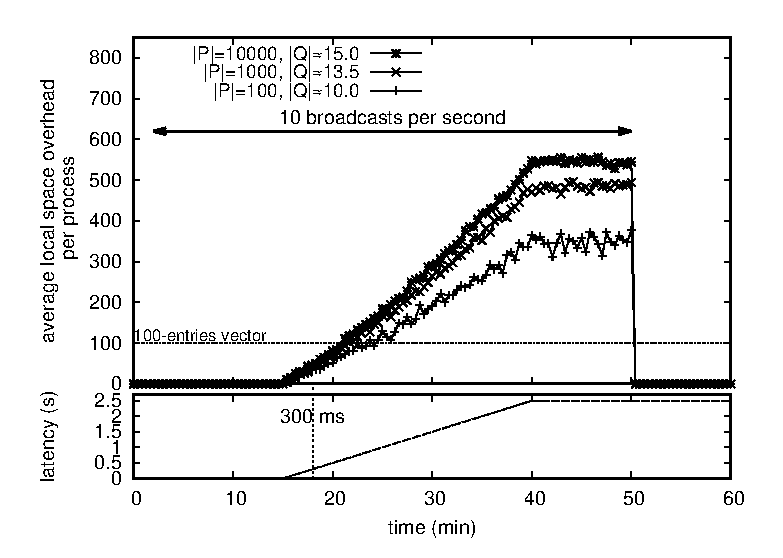
\includegraphics[width=1.0\textwidth]{img/overhead.eps}

\end{frame}


\begin{frame}{Experiments: small traffic overhead}

  \hspace{-1em}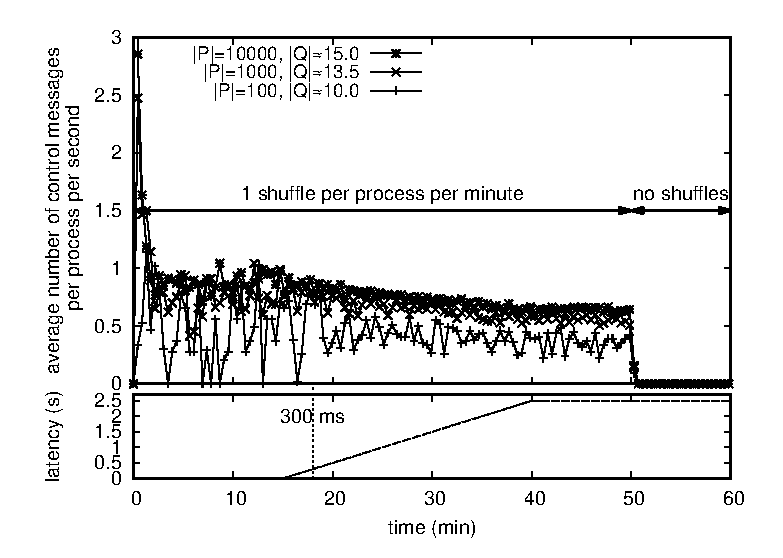
\includegraphics[width=1.0\textwidth]{img/controlmessages.eps}
    
\end{frame}


\begin{frame}{Conclusion}
  
  PRC-broadcast constitutes a new trade-off for causal broadcast.

  \vspace{2em}

  \begin{table}
    \begin{center}
      
\setlength{\tabcolsep}{4pt} % General space between cols (6pt standard)

\small

\begin{tabularx}{0.98\columnwidth}{@{}Xcccc@{}}
  & \makecell{message\\overhead} &  \makecell{delivery\\execution time} & \makecell{local space\\consumption} & \makecell{\# control messages\\per added link} \\ \cmidrule{2-5}
  vector-based R-broadcast & $O(1)$ & $O(1)$ & $O(\NO{N})$ & $0$ \\
  vector-based C-broadcast & $O(\NO{N})$ & $O(W.\NO{N})$ & $O(\NO{N}+W.\NO{N})$ & $0$ \\ 
  \footnotesize{PC-broadcast} & $O(1)$ & $O(1)$ & $O(\NO{N})$ & $3$ to \NO{$2P^2$} \\ \hline\hline
  \scriptsize{PRC-broadcast} & $O(1)$ & $O(Q_i)$ & $\mathbf{O(Q_i.M)}$ & $\mathbf{6}$ to $\NO{\mathbf{4P^2}}$ \\
%  \bottomrule
\end{tabularx}

%%% Local Variables:
%%% mode: latex
%%% TeX-master: "../paper"
%%% End:

    \end{center}
  \end{table}

  \vspace{2em}

  \faLightbulbO~Fun fact! This implementation of causal broadcast even makes an
  efficient implementation for reliable broadcast!

\end{frame}


\begin{frame}[standout]

  To be continued\ldots Retrieving partial order out of flattened orders.
  
  \vspace{2em}
  
  \begin{center}
    
\begin{tikzpicture}[scale=1]

%\normal

\newcommand\Y{-25pt};
\newcommand\X{25pt};
  
\draw[fill=black] (0, 0*\Y) node[left]{\footnotesize$a$} circle (1pt);
\draw[->](0*\X, 0*\Y) -- (0, 1*\Y);
\draw[fill=black] (0, 1*\Y) node[left]{\footnotesize$b$} circle (1pt);
\draw[->](0, 1*\Y) -- (0, 2*\Y);
\draw[fill=black] (0, 2*\Y) node[left]{\footnotesize$a'$} circle (1pt);

\draw[->] ( 1*\X, 1*\Y) -- ( 2*\X, 1*\Y);

\draw[fill=black] (3*\X, 0*\Y) node[left]{\footnotesize$a$} circle (1pt);
\draw[->](3*\X, 0*\Y) -- (3*\X, 1*\Y);
\draw[fill=black] (3*\X, 1*\Y) node[left]{\footnotesize$b$} circle (1pt);
\draw[->](3*\X, 0*\Y) -- (4*\X, 1*\Y);
\draw[fill=black] (4*\X, 1*\Y) node[right]{\footnotesize$a'$} circle (1pt);




\end{tikzpicture}
  \end{center}
  
\end{frame}


\begin{frame}[standout]

  \vspace{6em}
  
  Thanks!

  \vspace{5em}

  \small
  \faEnvelope ~ brice.nedelec@ls2n.fr

\end{frame}

\end{document}
